\chapter{Orígens del Bluetooth Low Energy}\label{C:compaginacio}

\section{Ús lliure de radiofreqüència}
En tot l'espai radioelèctric hi ha certs trams que estan assignats per a un ús lliure i privat.
Per utilitzar-los és necessari respectar la normativa nacional que normalment assimila la normativa comuna segons la ITU\footnote{La Internation Telecomunications Union depèn de les nacions unides i s'encarrega d'assignar l'espectre radioelèctric per a comunicacions.}.
Aquestes bandes es designen ISM, acrònim d'\textit{Industrial}, \textit{Scientific} i \textit{Medical}, que són els usos pels quals s'havia pensat que servirien originalment, avui en dia aquests usos són més diversos.

Com que les bandes ISM estan suficientment establertes arreu del món es crea la possibilitat d'utilitzar la comunicació sense fils amb molta facilitat pel públic general.
Aquesta situació proporciona el disseny de productes per al consumidor habitual que ràpidament veu els avantatges de la comunicació sense fils entre dispositius.
En aquest entorn sorgeix la necessitat d'establir estàndards entre companyies que veuen el benefici de proporcionar intercompatibilitat.
Per definir els estàndards les companyies s'agrupen i formen grups com la WI-FI Alliance o el NFC Forum.

\section{Bluetoooth}
Bluetooth és un estàndard per l'intercanvi de dades de curt abast que utilitza la banda ISM de 2,4 GHz.
És un dels protocols més coneguts i utilitzats, sobretot a través dels dispositius mòbils.
A continuació, s'explicarà l'origen d'aquesta tecnologia.

\subsection{Història de Bluetooth Clàssic}
El desenvolupament de la tecnologia per a connexions de curt abast que acabarien esdevenint el que avui es coneix com a Bluetooth Clàssic va començar l'any 1989 per part de l'empresa Ericsson.
Inicialment l'objectiu d'aquesta tecnologia era poder connectar auriculars i ordinadors sense necessitat d'una connexió per cable.
D'altra banda a IBM es volia integrar la connectivitat de la xarxa de telefonia als ordinadors portàtils per poder realitzar i rebre trucades des d'aquests mateixos.
El problema era que, això suposava un consum d'energia significatiu en els ordinadors portàtils de l'època.

IBM va veure que la tecnologia que estava desenvolupant Ericsson podria servir per tenir connectivitat de telefonia en els portàtils si es connectava el telèfon mòbil amb l'ordinador.
Preveient que la mobilitat en el futur seria important, les dues empreses van acordar utilitzar aquesta tecnologia en els seus productes corresponents.
El resultat va ser que els mòbils Ericsson i els ordinadors ThinkPad es podien comunicar entre si, i va permetre realitzar trucades des del portàtil.
Com que ni Ericsson ni IBM tenien majoria en la quota de mercat dels respectius productes van decidir que la tecnologia fos oberta.
D'aquesta manera es buscava integrar a més participants en aquesta tecnologia per tal de fer-la compatible amb la majoria de dispositius possibles.
El 1998 es van unir al grup Intel, Nokia i Toshiba i totes 5 companyies van fundar el Bluetooth SIG (\textit{Bluetooth Special Interest Group}, d'ara endavant SIG).
Finalment, al 2001 van sortir a la venda els primers dispositius amb Bluetooth, el terminal Ericsson T39 i el portàtil IBM ThinkPad A30.

\subsection{Història de Bluetooth Low Energy}
Com que el món de les comunicacions estava evolucionant cap als dispositius sense fils i alimentats amb bateria, era important adaptar les tecnologies existents per a les noves necessitats.
L'any 2001 a Nokia es va començar a desenvolupar una versió de Bluetooth que fos similar però que reduís significativament el consum d'energia amb el mínim de compromisos possibles.
Aquest desenvolupament va culminar l'any 2004 amb la publicació de la \textit{Bluetooth Low End Extension} \cite{Original_BLE_Extension}. 
Posteriorment, es va dur a terme múltiples millores juntament amb Logitech en el projecte d'investigació per part de la Unió Europea MIMOSA \cite{MIMOSA}.
El resultat del projecte es va anunciar el 2006 amb el nom de Wibree, es pot veure el logo a la Figura \ref{wibree_logo}.

\begin{figure}[hb]
	\begin{center}
		
\includegraphics[width=0.6\textwidth]{./images/Wibree_Logo.png}
		\caption{Logo de Wibree}
		\label{wibree_logo}
	\end{center}
\end{figure}

Els membres del SIG després de negociar entre si, van acordar incloure Wibree l'estàndard de Bluetooth en l'especificació 4.0 amb el nom de \textit{Bluetooth ultra low power technology} i publicitat com a Bluetooth Smart. El primer mòbil a incloure'l va ser l'iPhone 4S que va sortir al mercat el 2011.
Posteriorment es va canviar el nom per \textit{Bluetooth Low Energy} (BLE d'ara endavant).

\section{Bluetooth Clàssic vs BLE}
El Bluetooth Low Energy no té cap relació amb el Bluetooth Clàssic pel que fa a l'arquitectura de la tecnologia.
Tot i que comparteixen l'ús de la banda freqüencial de 2,4 GHz i contenen el nom de Bluetooth, són completament diferents, de fet, no són compatibles entre si.
Quan un dispositiu vol implementar les dues tecnologies (anomenat mode dual) ho ha de fer per separat, ja que només comparteixen l'antena; les modulacions i els altres blocs són tots diferents.

\section{MANETS (\textit{Mobile Ad-Hoc Networks})}
Bluetooth Clàssic no permet tenir més d'una connexió establerta amb altres dispositius.
A més a més té el desavantatge que, tot i voler transmetre poques dades, l'arquitectura fa que es consumeixi força energia per establir i mantenir la connexió, encara que sigui breu.
Això no suposava problemes inicialment, ja que l'ús principal era per la transferència de fitxers petits com contactes o fotografies.
Més endavant també es va fer popular l'us del Bluetooth per a escoltar música a través d'auriculars sense fils.
En aquests casos el cost d'establiment de la connexió és insignificant en comparació amb el cost mentre s'estan transferint dades, que acostuma a ser un període llarg de temps.
Posteriorment, amb l'ús dels telèfons intel·ligents i l'augment del consum de continguts, sobretot música, es va millorar Bluetooth per ser més resistent a interferències i aconseguir velocitats superiors i així poder transmetre música d'alta fidelitat.

D'altra banda, va començar a sorgir l'Internet of Things, basat a tenir molts dispositius connectats, transmetent a taxes molt variades i de forma discontínua.
Això va generar necessitats que no es podien cobrir amb les tecnologies existents.
Era necessari tenir xarxes sense fils, amb consum molt baix d'energia i que cobrissin una gran distància (10-100 metres).
Amb aquests requeriments, van sorgir les xarxes ad hoc o \textit{Mobile Ad-Hoc Networks} (MANETS d'ara endavant).

\subsection{Altres MANETS}
\label{MANETS}
BLE és una de les MANETs més populars però n'hi ha d'altres que competeixen i que es detallaran a continuació.

\subsubsection{Zigbee}
L'estàndard Zigbee s'utilitza en entorns per l'automatització de la casa, xarxes de sensors, col·lecció de dades mèdiques entre d'altres.
Zigbee està dissenyat per sobre de l'IEEE 802.15.4\footnotemark{} i per tant, només defineix les capes superiors.
No està pensat per a situacions amb gran mobilitat entre nodes sinó per a desplegaments més estàtics.
Aquesta tecnologia, per exemple, s'utilitza en els dispositius de Philips Hue que serveixen per controlar bombetes intel·ligents.

\subsubsection{6LoWPAN}
IPv6 \textit{over Low power Wireless Personal Area Networks} és un protocol que permet enviar paquets d'Internet Protocol versió 6 (IPv6) a través de l'IEEE 802.15.4\footnotemark[\value{footnote}].
Aquest protocol està orientat a aportar Internet amb connexions sense fils.
Una de les característiques destacades és la capacitat de comprimir les capçaleres dels paquets per així reduir el sobrecost que suposa.
La utilització del 6LoWPAN és majoritàriament coneguda per l'estandardització del protocol Thread que l'utilitza per a domòtica.

\footnotetext{L'IEEE 802.15.4 és un estandàrd orientat a xarxes sense fils amb una baixa taxa de dades. Aquest només defineix les capes físiques i d'accés al medi.}

\subsubsection{Z-Wave}
Z-Wave és un protocol utilitzat principalment en domòtica. La comunicació es fa en una xarxa en malla que connecta els electrodomèstics i per tant, permet el seu control.
La principal característica d'aquest protocol és que utilitza únicament les freqüències ISM de la banda 800 o 900 MHz (segons continent) i així evita les interferències que hi ha a 2.4 GHz de WIFI o Bluetooth.
La utilització de freqüències més baixes permet més abast amb menys potència, especialment quan es tracta de penetrar parets.
Un exemple de dispositius que utilitzen aquesta tecnologia són els productes de la marca Ring principalment coneguts pels seus vídeo-porters intel·ligents.

\subsubsection{Insteon}
Insteon està orientat a domòtica i utilitza conjuntament radiofreqüència i les línies d'alimentació de casa per a la comunicació.
Aquest tipus de sistema s'anomena de malla dual.
El fet d'estar connectats tots els dispositius a la instal·lació elèctrica facilita una molt bona sincronització entre els dispositius.
Això permet, per exemple, que múltiples dispositius puguin retransmetre paquets alhora per tal de millorar la cobertura i reduir les retransmissions.
SmartLabs és la companyia que fabrica i ven els productes que utilitzen Insteon.

\subsubsection{LoRa}
El protocol Long Range desenvolupat per Semtech està orientat a cobrir les distàncies més grans d'entre les MANETs.
Ho aconsegueix reduint la taxa de transmissió de dades reals, augmentant així, el temps dedicat a cada símbol donant més oportunitats al receptor per detectar correctament el senyal.
Aquesta tècnica s'anomena espectre eixamplat i LoRa la implementa amb \textit{Chirps}.
Els \textit{Chirps} són els polsos que es transmeten, sempre s'envien més \textit{Chirps} que bits i la relació ve definida pel factor d'eixamplat o \textit{Spreading Factor}.
LoRa permet configurar aquest paràmetre que defineix l'equilibri entre la taxa de dades i la distància, pot prendre valors entre 7 i 12.
El LoRa també implementa protecció contra errors o FEC (\textit{Forward Error Correction}) per incrementar encara més l'abast.

Pel que fa a la pila de protocols que s'utilitzen en la comunicació, LoRa únicament defineix les capes inferiors.
Això suposa que només s'ha especificat com funciona la modulació dels senyals analògics i com es transformen en símbols digitals.
Tot i així, la LoRa Alliance va definir el LoRaWAN que és un dels protocols que es poden utilitzar per a les capes superiors.


\subsection{Comparació}
Tot i que els protocols tenen molt en comú, com per exemple el se ús en domòtica, cadascun es diferencia de la resta en els detalls.
A la taula \ref{taula_comparacio} es pot veure una comparació de les capacitats de cada un dels protocols.
Cal mencionar que les freqüències de les bandes mencionades poden variar lleugeramanet segons la normativa de cada país.
En la comparació es pot veure com BLE és una de les que té millors capacitats.
Això es deu al fet que tot i que no és possible aconseguir totes les característiques alhora la seva flexibilitat permet configurar el protocol per a moltes configuracions diferents.

\begin{table}[h]
	\centering
	\resizebox{\textwidth}{!}{
		\begin{tabular}{|r|c|c|c|c|c|}
			\hline
&Abast (m)&	Velocitat Física (Kbps)	&	Taxa de dades (Kbps)   & Consum (mA) & Banda\footnotemark   \\ \hline
BLE 4	&	50		& 1000	& 800  	& 15	& 2.4 GHz		\\ \hline
BLE 5	&	200 	& 2000	& 1430 	& 15	& 2.4 GHz		\\	\hline
6LoWPAN	&	100    	& 250 	& 162	& 15	& 900 MHz i 2.4  GHz		\\	\hline
Zigbee	&	100		& 250	& 162 	& 30	& 900 MHz i 2.4  GHz        \\	\hline
Z-Wave	&	90 		& 100	& 40  	& 23	& 900 MHz	\\	\hline
Insteon	&	120		& 4,5	& 2,8	& --	& 915 MHz		\\	\hline
LoRa	&	10 Km	& 50	& 5		& 18	& 400 i 900 MHz				\\	\hline	
		\end{tabular}
	}
\caption{Comparació entre MANETs \cite{manets}}
\label{taula_comparacio}
\end{table}

\newpage
\footnotetext{Les bandes freqüencials indicades com a 900 MHz varien depenent del país entre 800 MHz i 1000 MHz}

\section{Versions de BLE}
\label{Versions_BLE}
Tal com s'ha vist anteriorment, BLE és classifica segons les seves capacitats en la seva versió 4 i en la 5.
Això és deu als canvis significatius que ha experimentat aquesta tecnologia en les últimes versions \cite{BLE_5_improvement_over_4}.
Les novetats que aporta la nova versió principalment tenen l'objectiu d'incrementar les capacitats del protocol en els casos extrems, tant en entorns molt favorables com quan no són favorables.
Les millores i noves opcions de BLE fan que s'utilitzi més eficientment l'espectre freqüencial i per tant, depenent de la regió, es pugui augmentar la potència de transmissió de 10 dBm, que era el límit de BLE 4.2, a 20 dBm en BLE 5.

\subsubsection{LE 2M}
\textit{Low Energy 2 Mega} (LE 2M) és el nom que té la nova capa física, que és opcional, quan opera a 2 MBd\footnote{El Baud (Bd) és la unitat de mesura de la velocitat de modulació, que correspon al nombre de canvis de l'estat d'un senyal en un segon.} en la versió 5 en lloc dels 1 MBd que era l'única opció en la versió 4.
L'augment de la velocitat dels símbols permet incrementar la quantitat de dades que es poden transmetre a nivell d'aplicació.
Aquest canvi està pensat per facilitar la utilització de BLE en situacions més exigents pel que fa a volum de dades com per exemple, múltiples mesures del cos humà.
 
\subsubsection{Abast}
Tot i que la tecnologia BLE en la seva versió original (4.0) tenia una distància màxima de transmissió teòrica molt gran (100 metres sense obstacles), no era suficient per a tots els casos.
Per exemple, era necessari tenir més abast en els sectors com el de les cases intel·ligents que tenien un abast real relativament baix degut als obstacles entre dispositius.
El límit de l'abast, en part, ve definit per la potència màxima de transmissió (sigui per protocol o per normativa) i per la probabilitat d'error de bit BER (\textit{Bit Error Ratio}) que es pot tolerar.
Bluetooth defineix la BER màxima en 0.1\% per tant quan un de cada mil bits és erroni es considera que la connexió és massa dolenta i que ja s'ha arribat al límit de distància.

Per tractar els errors en transmissió hi ha dues estratègies: detecció d'errors i correcció d'errors.
En la versió 4.0 de Bluetooth només s'utilitzava la detecció d'errors, en canvi, en Bluetooth 5 s'implementa la correcció d'errors.
D'aquesta manera sense augmentar la potència transmesa es pot incrementar l'abast màxim que pot tenir la comunicació.
El desavantatge és que més bits dels que es transmeten es dediquen a redundància per tant queda menys espai per a dades de l'aplicació.


L'esquema de correcció d'errors (\textit{Forward Error Correction}) es fa amb un codificador convolucional que pot generar a la sortida més bits dels que entren. El codificador pot funcionar amb dos esquemes diferents s'anomenen $S=2$ i $S=8$.
Amb els diferents esquemes s'utilitza una taxa de codi diferent que pot augmentar la capacitat de correcció i incrementar l'abast però disminuir la quantitat de dades que es poden transmetre.
Es poden veure les capacitats dels diferents esquemes a la taula \ref{FEC}.

\begin{table}[htb]
	\begin{center}
		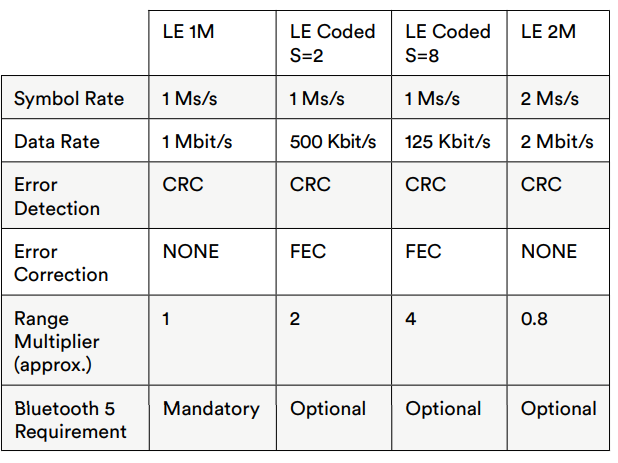
\includegraphics[width=0.8\textwidth]{./images/LE_PHY_edited.png}
		\caption{Comparació de diferents capes físiques \cite{BLE_5_improvement_over_4}}
		\label{FEC}
	\end{center}
\end{table}

\subsubsection{Advertisement Extensions}
\label{Advertisement_Extensions}
En Bluetooth 4.0 els paquets d'anunci (\textit{Advertisement Packets}) tenen 6 octets de capçalera i com a molt 31 de dades, és a dir, com a molt es poden transmetre 31 Bytes de cop.
Normalment, aquests paquets es transmeten pels 3 canals d'anuncis el 37, 38 i 39.

En Bluetooth 5 per poder difondre (\textit{broadcast}) més dades el que es fa és enviar un paquet d'anunci on només s'indica la capçalera i un punter cap al canal per on s'enviarà el paquet complet.
Posteriorment, pel canal per on s'ha indicat s'envia el paquet de dades i en cas de necessitar més dades s'encadenen paquets.
D'aquesta manera, les dades només es transmeten una vegada, ja que abans, calia transmetre-les en els tres canals d'anunci.
Aquest procediment està detallat més endavant en l'apartat  \ref{Advertising_Extension_PDU}

En la versió 4.0 quan es vol enviar un paquet és necessari esperar un cert temps aleatori.
Aquest procediment evita les col·lisions periòdiques però suposa que els dispositius han d'estar durant més temps escoltant, ja que no saben quan rebran el paquet exactament.
En BLE 5 el GAP, que s'explicarà en profunditat a l'apartat \ref{GAP}, defineix un mode síncron que permet utilitzar un procediment d'establiment d'anunciaments sincronitzats.
També existeix una nova capçalera \textit{SyncInfo} on s'indica amb exactitud l'interval i variació dels paquets.
Així doncs, s'aconsegueix evitar les col·lisions i reduir el temps que el dispositiu ha de tenir la ràdio encesa.

\subsubsection{Slot Availability Masks}
La tecnologia LTE (telefonia) està utilitzant cada vegada més espai freqüencial i en preparació de que s'utilitzi en freqüencials pròximes a la banda de 2.4 GHz ISM s'ha desenvolupat un sistema per indicar disponibilitat en el temps.
Per evitar les possibles interferències que causin altres tecnologies, es defineix la SAM (\textit{Slot Availability Mask}) que permet identificar aquelles ranures de temps on hi ha disponibilitat així bloquejant aquells moments on hi hagi interferències per evitar-les.

\subsubsection{Improved Frequency Hopping}
Els salts en freqüència que utilitza la versió 4.0 estan definits per 12 seqüències predeterminades.
En canvi, BLE 5 utilitza una seqüència pseudo-aleatòria per determinar quins canals s'utilitzen.
L'algorisme, en aquest cas, és el \textit{channel selection algorithm \#2} i és més efectiu a evitar interferències i esvaniments per propagació multicamí.

\section{Pila BLE}
Un cop vistes les característiques generals del protocol cal entendre com funciona per dins.
A continuació, es descriurà la pila de BLE i es veurà cada una de les capes que en formen part i les seves funcions.

\begin{figure}[h!]
	\begin{center}
		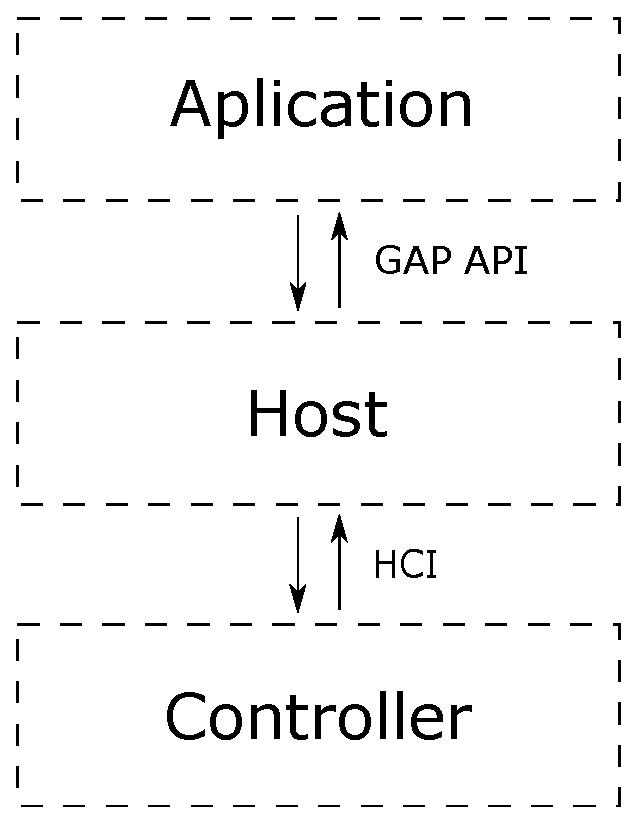
\includegraphics[width=0.4\textwidth]{./diagrames/BLE_Stack_Simplified}
		\caption{Pila de BLE}
		\label{ble_stack}
	\end{center}
\end{figure}

La pila pròpia de Bluetooth Low Energy està dividida en dues parts, tal com es pot observar a la Figura \ref{ble_stack}, el controlador i el \textit{host}. Aquestes dues parts són independents i utilitzen el protocol \textit{Host Controller Interface} (HCI d'ara endavant) per comunicar-se entre elles.
Aquest protocol pot estar implementat amb qualsevol protocol de transport físic com USB o UART.
La idea darrera de separar la pila en dos serveix per fer compatibles xips fets per diferents fabricants.
Les dues parts de la pila poden ser implementades en el mateix xip anomenat configuració única o en xips separats anomenat configuració dual.


\subsection{Controller}
El controlador compren la capa física i la capa d'enllaç en l'ordre que mostra la Figura \ref{controller_stack}.

\begin{figure}[h!]
	\begin{center}
		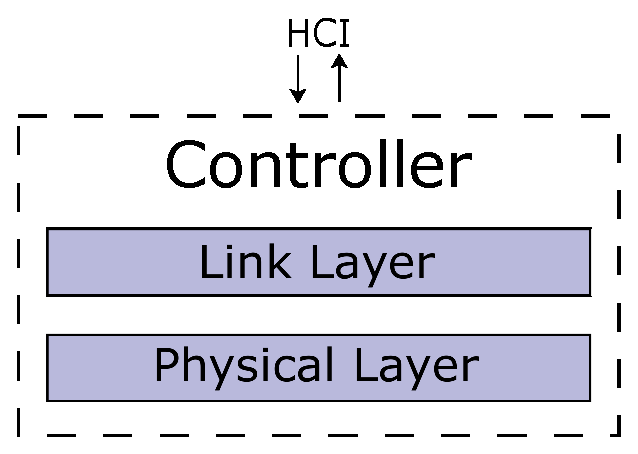
\includegraphics[width=0.4\textwidth]{./diagrames/BLE_Controller}
		\caption{Controller Stack}
		\label{controller_stack}
	\end{center}
\end{figure}

\subsubsection{Capa Física}
La capa física és la que s'encarrega de la comunicació anal·lògica modulant i desmodulant els senyals.
Tal i com ja s'ha comentat abans, treballa a la banda de 2.4 GHz en 40 canals diferents tal i com es mostra a la Figura \ref{BLE_Channels}.

\begin{figure}[hb]
	\begin{center}
		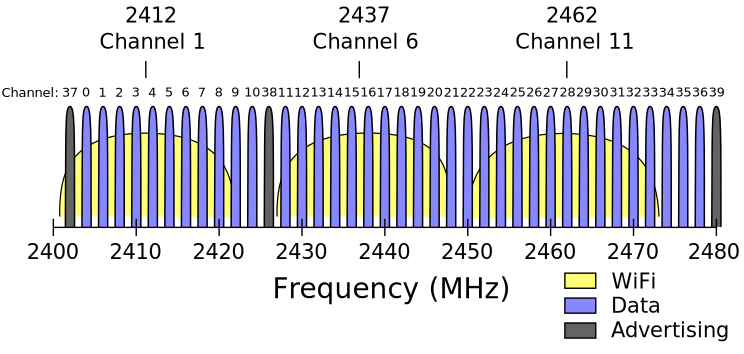
\includegraphics[width=0.8\textwidth]{./diagrames/BLE_WiFi}
		\caption{Canals BLE \cite{ble_feq}}
		\label{BLE_Channels}
	\end{center}
\end{figure}

Els canals es classifiquen en 37 de dades o també anomenats secundaris i 3 d'anunci (\textit{Advertisment}) o primaris.
En els canals d'anunci es vol tenir més qualitat, ja que la informació que s'hi transmet és més important.
Per exemple, són els canals que s'utilitzen per descobrir altres dispositius.
És per això, que els canals d'anunci es troben en el buits que deixen els canals WiFi més comuns (1, 6 i 11), tal com es veu a la Figura \ref{BLE_Channels}.

El protocol BLE té l'objectiu de consumir el mínim d'energia possible, això es pot millorar reduint el temps que s'està transmetent o escoltant a través de la ràdio.
Si no s'ha de rebre o transmetre res, es pot apagar la ràdio i s'estalvia energia.
El BLE és un dels protocols que tenen la taxa de transmissió física \footnote{La taxa de transmissió física és aquella a la que transmeten la ràdio, no confondre amb la taxa de dades d'aplicació \textit{Throughput}} més alta, i de fins a 1 Mbps originalment i de 2 Mbps en BLE 5.

La potència màxima de transmissió és de 20 dBm (100 mW) segons l'especificació\footnote{La PCB utilitzada pot transmetre fins a 5 dBm de potència}.
Aquesta potència de la ràdio es pot controlar, disminuint-la per consumir menys energia.
Tot i que això, només serà possible si l'entorn ho permet i el receptor pot rebre el senyal correctament.
Els paquets de BLE indiquen la potència amb que s'han transmès i junt amb el RSSI (\textit{Received Signal Strength Indicator}), la potència rebuda, es pot estimar la distància fins al transmissor.
Conèixer aquest valor és útil per a certes aplicacions, per exemple, la localització en espais interiors.

La modulació utilitzada per BLE és la GFSK (\textit{Gaussian Frequency Shift Keying}), aquesta modulació és una de les més robustes, simples d'implementar i és el que permet a BLE, en part, tenir un abast molt més gran que Bluetooth Clàssic.
El filtre gaussià redueix el consum pic d'energia \cite{BLE_Review} i també redueix les interferències en freqüències veïnes.
En BLE 4.0 s'utilitza una desviació freqüencial de 185 kHz, en BLE 5 com que augmenta la velocitat de símbols també creix la interferència intersimbòlica.
Per mitigar aquest efecte negatiu, la desviació de freqüència passa a ser de 370 kHz.


\subsubsection{Link Layer}
La capa d'enllaç és l'encarregada d'escanejar, anunciar i gestionar les connexions amb altres dispositius.

\begin{figure}[!h]
	\begin{center}
		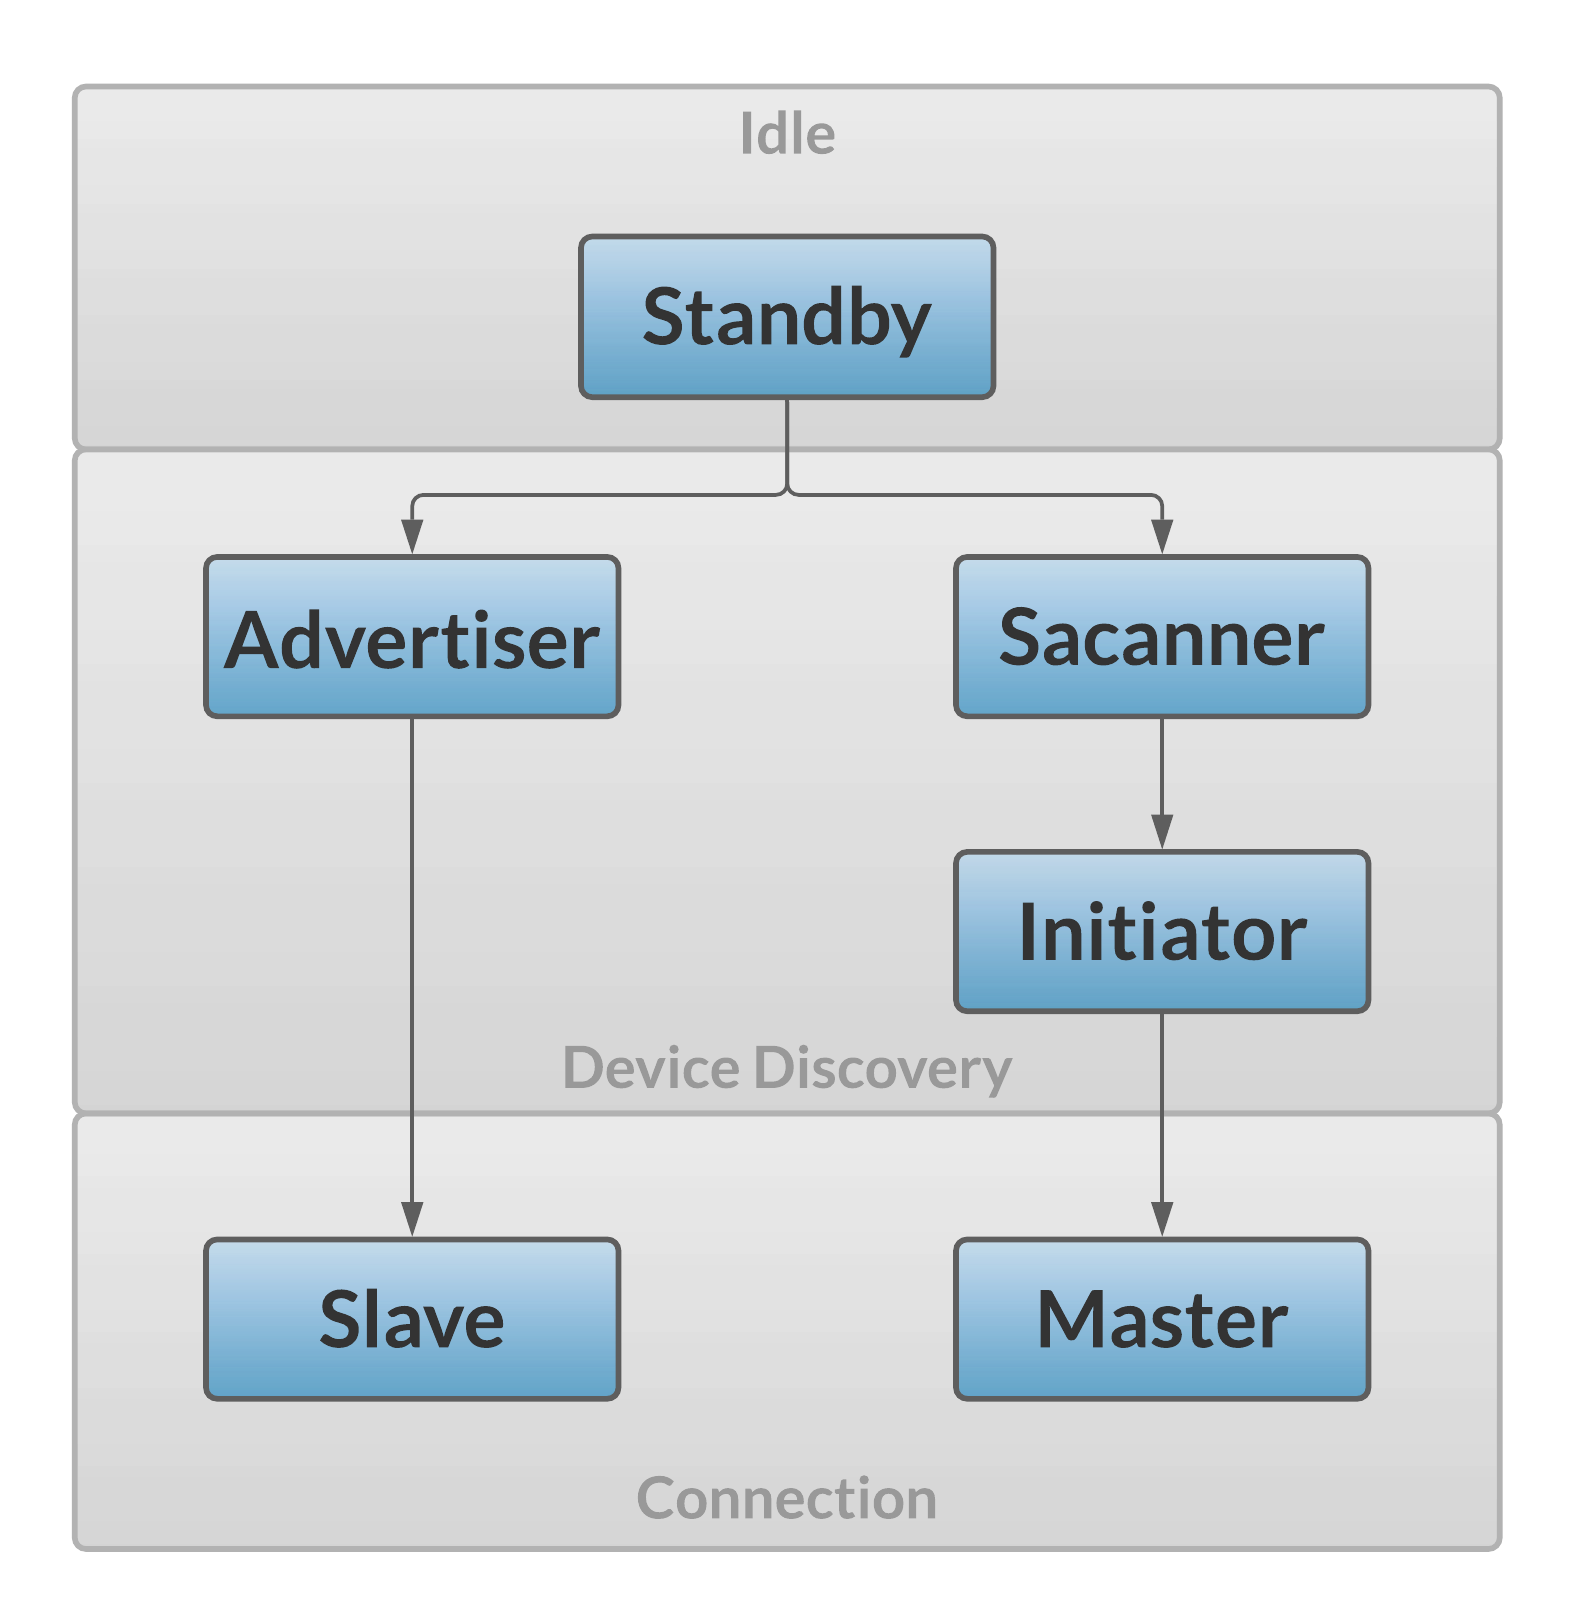
\includegraphics[width=0.6\textwidth]{./images/link_state_diagram.png}
		\caption{Estats de la capa d'enllaç \cite{Link_Layer_states}}
		\label{Link_State_Diagram}
	\end{center}
\end{figure}

Depenent del moment en la connexió, els dispositius es troben en diferents estats.
Els estats son: Espera (\textit{Standby}), Anunciador (\textit{Advertiser}) o Escàner (\textit{Scanner}) i Iniciador (\textit{Initiator}), Esclau (\textit{Slave}) o Mestre (\textit{Master}).
A la Figura \ref{Link_State_Diagram} s'hi pot veure el flux d'estats per arribar a una connexió.

Aquesta capa és l'encarregada d'implementar el salt en freqüència (\textit{frequency hopping}) que permet mitigar l'impacte de les interferències estretes.
Si s'utilitzés només un dels canals BLE i en aquell canal hi haguessin interferències no es podria establir comunicació.
Al alternar múltiples canals, encara que hi hagi interferències en algun d'ells es considera que no n'hi haurà en tots i per tant hi podrà haver una bona comunicació.
Els salts que es fan són des de 5 fins 16 canals per salt d'entre els dedicats a dades.

\subsection{Host}
El protocol BLE es va dissenyar amb la flexibilitat en ment, és per això que l'estructura de la pila del host permet no utilitzar certes capes que es consideren opcionals tal com es pot veure a la Figura \ref{host_stack}.
El permetre tenir capes opcionals pot generar incompatibilitats entre dispositius però no és comú.
En canvi, facilita molt i abarateix el disseny d'un dispositiu BLE en cas que no es necessitin totes les capacitats que ofereix.

\begin{figure}[h!]
	\begin{center}
		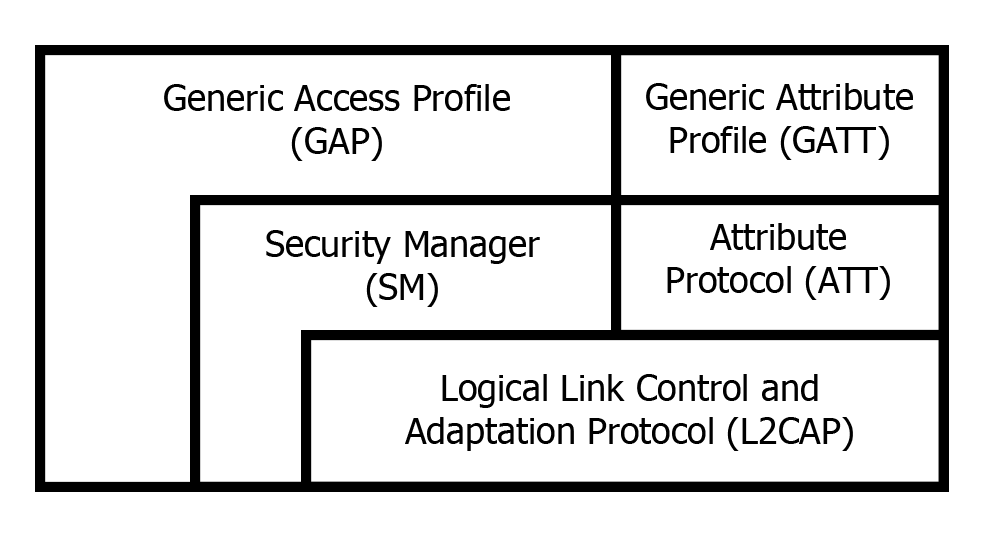
\includegraphics[width=0.8\textwidth]{./images/ble_host_stack.png}
		\caption{Pila del Host \cite{ble_stack}}
			\label{host_stack}
	\end{center}
\end{figure}

\subsubsection{L2CAP (\textit{Logical Link Control and Adaptation Protocol})}
La \textit{Logical Link Control and Adaptation Protocol} és la capa encarregada de l'establiment de la connexió lògica; segmentació i reassemblatge de paquets; multiplexament de protocols;  i control de flux individual per canal.

La multiplexació de protocols és necessària per aconseguir que BLE sigui flexible.
Permet que des de capes superiors s'utilitzin els protocols que necessiti el fabricant, i no només aquells determinats per l'estàndard de BLE.

Degut a la limitació física de l'arquitectura, existeix una MTU\footnote{La MTU és la mida màxima que pot tenir un paquet} (\textit{Maximum Transmission Unit}) i per tant és necessari segmentar els paquets de les capes superiors que es converteixen en paquets més petits per a les capes inferiors.
Aquesta MTU es pot definir (dins dels límits establerts) independentment per cada connexió així flexibilitzant l'ús que es dóna al protocol en cada cas.
La L2CAP també és la capa que fa el seguiment de la qualitat de la connexió i dels recursos utilitzats per assegurar-se que les necessitats dels serveis es compleixen.

\subsubsection{\textit{Security Manager}}
La capa \textit{Security Manager} o SM proveeix de diferents serveis relacionats amb la seguretat de la connexió.
Aquests serveis són: autenticació i autorització de dispositius; i també integritat, confidencialitat i privacitat de les dades.
El protocol té flexibilitat en el tipus d'emparellament i la generació de claus per aconseguir reduir els requeriments de memòria i energia segons les necessitats específiques.
Els diferents mètodes de seguretat es comentaran en més profunditat a l'apartat \ref{sec:security}

\subsubsection{ATT \& GATT}
L'\textit{Attribute Protocol} (ATT d'ara endavant) és el protocol d'aplicació més comú per a BLE i el \textit{Generic Attribute Profile} (GATT d'ara endavant) defineix com utilitzar el protocol per oferir serveis a capes superiors.
L'ATT és un protocol dissenyat per a dispositius \textit{Low Energy} amb l'objectiu de minimitzar la quantitat de dades transmeses. L'atribut està format per 4 elements, \textit{handle}, UUID, permisos  i \textit{value}.

El \textit{handle} fa la distinció única entre els diferents atributs, ocupa 16 bits i habitualment els valors són seqüencials. És molt útil, ja que s'utilitza per referenciar l'atribut amb el mínim de bits possibles.
L'UUID (\textit{Universal Unique IDentifier}) identifica el tipus d'atribut, aquest número pot ser de 16 bits si s'utilitza algun que ja està estandarditzat pel SIG o bé en tindrà 128 bits si està definit pel fabricant.
En els permisos s'indicarà quin tipus d'accés té el client a la informació (només lectura, lectura i escriptura ...). També pot estar definit si requereix un nivell mínim d'encriptació o si és necessari l'autenticació.
Finalment, el valor de l'atribut serà on hi ha la informació, la seva interpretació i longitud (512 bytes com a molt) dependrà de l'UUID.

\begin{figure}[h!]
	\begin{center}
		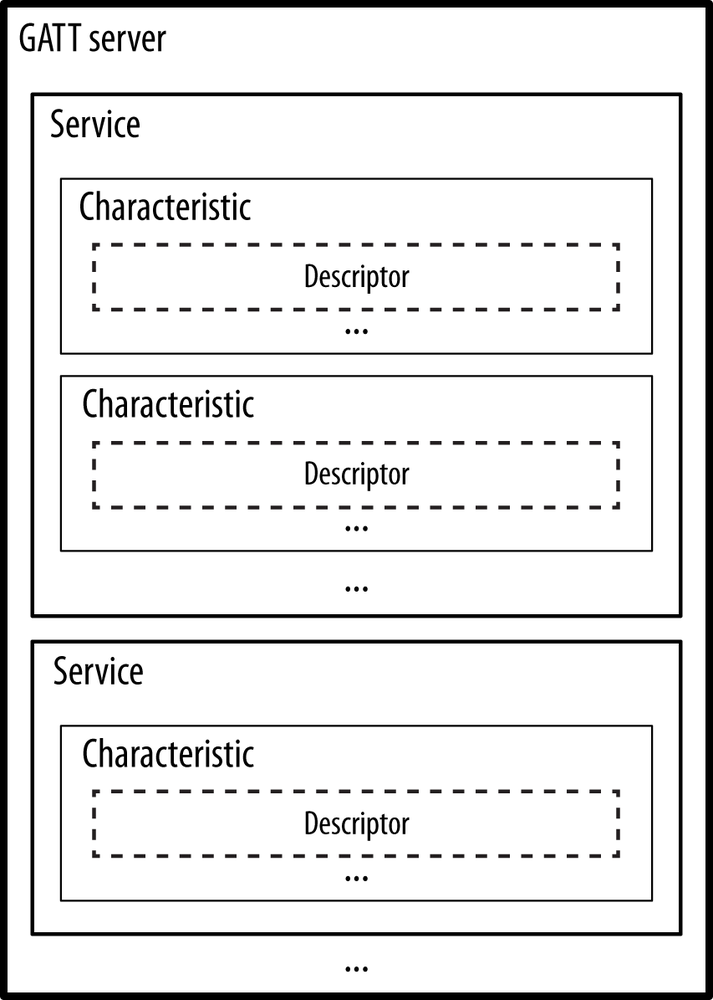
\includegraphics[width=0.4\textwidth]{./images/GATT_Hierarchy.png}
		\caption{Jerarquia de GATT \cite{GATT_Hierarchy}}
		\label{fig:Gatt_Hierarchy}
	\end{center}
\end{figure}

Des de la perspectiva del GATT els dispositius són clients i servidors.
Habitualment és el client qui pren la iniciativa demanant dades, tot i així, el servidor també té la capacitat d'iniciar una comunicació per exemple notificant quan un valor ha canviat.

La definició de l'ATT és massa genèrica per si sola tal que seria comú que, per fer el mateix, es desenvolupessin múltiples definicions que fossin incompatibles entre si.
Per tal de tenir millor definits els serveis s'utilitza el GATT.
El GATT permet definir perfils que agrupen múltiples atributs en un sol servei \cite{services}, la seva jerarquia es mostra en la Figura \ref{fig:Gatt_Hierarchy}.

En un llistat d'atributs el GATT identifica els serveis tenint en compte que cada servei comença amb un atribut amb l'UUID 0x2800.
Aquest atribut amb UUID 0x2800 s'anomena Declaració de Servei i tots els atributs consecutius fins a una altra declaració de servei formen part d'aquest.
En la declaració de servei el camp ``valor'' indica l'UUID que identifica de quin servei es tracta.
Cada servei conté característiques \cite{characteristics} definides en els atributs amb UUID 0x2803.
Aquests tipus d'atributs s'anomenen Declaració de Característica.
El valor de la declaració de característica està format per un nou UUID que identifica la característica i per un \textit{handle}.
Aquest \textit{handle} correspon a l'atribut on hi ha les dades de la característica.

\begin{table}[h]
	\begin{center}
		\definecolor{lightred}{RGB}{255, 128, 128}
		\definecolor{lightyellow}{RGB}{238, 232, 170}
		\begin{tabular}{|l|l|l|l|}
			\hline
			\textbf{Handle}	&	\textbf{UUID}	&	\textbf{Descripció}						&	\textbf{Valor}		\\ 	\hline \rowcolor{lightred}
			0x0100	&	0x2800	&	Battery Service					&	UUID 0x180F	\\		\hline \rowcolor{lightyellow}
			0x0101	&	0x2803	&	Characteristic: Battery Level	&	\parbox[t]{4cm}{UUID 0x2A19	\\ Value handle: 0x0102}	\\	\hline
			0x0102	&	0x2A2B	&	Battery Value					&	20	\\	\hline	\rowcolor{lightred}
			0x0103	&	0x2800	&	Custom Temperature Service		&	UUID 	706676c8-3e49...	\\	\hline	\rowcolor{lightyellow}
			0x0104	&	0x2803	&	Characteristic: Temperature		&	\parbox[t]{4cm}{UUID 0x2A6E	\\ Value handle: 0x0105}	\\		\hline	
			0x0105	&	0x2A6E	&	Temperature Value				&	25.45	\\	\hline \rowcolor{lightyellow}
			0x0106	&	0x2803	&	Characteristic: date/time		&	\parbox[t]{4cm}{UUID 0x2A08	\\ Value handle: 0x0107}	\\		\hline
			0x0107	&	0x2A08	&	Date/Time						&	1/1/1980 12:00	\\
			\hline
		\end{tabular}	
		\caption{Exemple de possibles atributs}
		\label{Attribute_Table}
	\end{center}
\end{table}

En aquest exemple de la taula \ref{Attribute_Table} es pot observar que hi ha 2 serveis diferents, marcats en vermell, ja que hi ha 2 UUID 0x2800.
També es mostren 3 característiques en total, marcades en groc, (una pel primer servei i dues pel segon) que corresponen als 3 atributs amb UUID 0x2803.
Com que els valors corresponents al nivell de bateria i la temperatura estan estandarditzats (veure \cite{Battery_Level}\cite{Temperature_Characteristic}, respectivament), no cal especificar que es refereixen a percentatge de bateria restant i a graus Celsius.

En la declaració de servei de temperatura (\textit{Handle} 0x0103) es pot veure que no forma part de l'estàndard, ja que el seu valor té 128 bits.
S'ha escollit per a aquest projecte un UUID completament aleatori, en concret el 706676c8-3e49-4ecc-9379-fa9851444e53.
Aquest UUID identifica el servei que s'ha desenvolupat per l'exemple i en teoria hauria de ser únic.
No es pot saber amb seguretat que algun altre desenvolupador no hagi escollit el mateix UUID i no hi ha una coordinació establerta.
Tot i això es considera del tot improbable que es produeixin col·lisions gràcies a la longitud de 128 bits.

La condició que ha de complir l'UUID és que no acabi en 0000-1000-8000-00805F9B34FB, ja que aquest sufix correspon als que estan reservats segons l'estàndard.
És possible demanar al SIG tenir un UUID global reservat per a ús propi amb un cost de \$2.500.
Es poden veure tots els que ja s'han reservat oficialment a \cite{reservedUUIDs}.

En aquest exemple no n'hi ha cap però les característiques poden tenir descriptors \cite{descriptors} que permeten aportar informació addicional sobre la característica que els precedeix.
Aquests, per exemple, serveixen per poder subscriure's a rebre notificacions cada cop que una característica canvia de valor.
Els atributs també tenen propietats d'accés que defineixen quines accions es poden prendre.
Les propietats es comentaran en un exemple real més endavant \ref{sec:properties}

\subsubsection{GAP}
\label{GAP}
La \textit{Generic Access Profile} és la capa que interactua amb l'aplicació i per tant ofereix la Interfície de Programació d'Aplicacions (API en anglès) amb la funcionalitat que aporta BLE.

El dispositiu sempre està en un\footnote{En BLE 5.1 es permet certes combinacions de rols} dels quatre rols: Emissor, Observador, Perifèric o Central.
Si el rol és emissor, s'enviaran anuncis per poder ser descobert.
Si és Observador s'escoltaran els canals per obtenir informació dels anuncis.
Un cop s'estigui en una connexió el perifèric serà el node amb menys capacitats de processament o de bateria i és requerirà menys d'ell per mantenir la connexió, per exemple a un rellotge intel·ligent
En canvi el node Central serà el que tingui més recursos com pot ser un telèfon intel·ligent o un ordinador.
Amb aquests rols i l'especificació del GAP existeix l'estàndard que permet els dispositius descobrir-se, connectar-se i emparellar-se entre d'altres.


\section{Anunciaments}
Quan els dispositius volen transmetre informació o volen connectar-se entre si el primer que cal fer és anunciar-se.
BLE és molt flexible a l'hora de configurar els paràmetres d'anunci i permet al desenvolupador adaptar el protocol per a les necessitats que tingui.
A continuació, es concretarà quins són aquests paràmetres i com afecten les prestacions finals del sistema.

Els paquets d'anunci com ja s'ha explicat anteriorment són aquells que serveixen a un dispositiu per donar-se a conèixer i alhora opcionalment transmetre informació \cite{Advertising}.

\subsection{Tipus}
Existeixen 4 paquets d'aquest tipus i BLE 5 n'afegeix 4 més.
Els 4 originals es classifiquen segons si permet connexió i si permeten escaneig, tal com mostra la taula \ref{tab:Advertisment_Types}.

\begin{table}[!h]
	\begin{center}
		\begin{tabular}{|c|c|l|}
			\hline
			Connexió	&	Escaneig	&	Nom	\\	\hline
			Si			&	Si			&	ADV\_IND	\\	\hline
			Si			&	No			&	ADV\_DIRECT\_IND	\\	\hline
			No			&	No			&	ADV\_NONCONN\_IND	\\	\hline
			No			&	Si			&	ADV\_SCAN\_IND	\\	\hline
		\end{tabular}
	\end{center}
\caption{Tipus d'anunciaments}
\label{tab:Advertisment_Types}
\end{table}


L'ADV\_IND és el genèric, és el més comú i permet que qualsevol dispositiu pugui connectar-se.
L'ADV\_DIRECT\_IND serveix per anunciar-se a un dispositiu específic, per exemple, si un rellotge intel·ligent es vol connectar al telèfon al qual està associat.
L'ADV\_NONCONN\_IND només indica que existeix i no rebrà informació.
Això és útil, per exemple, per permetre localització de balises.
L'ADV\_SCAN\_IND també està orientat a balises però estarà escoltant per si rep missatges d'escaneig amb els que pot respondre amb poca informació.
Això permet una comunicació bidireccional limitada sense necessitat d'establir connexió.
Tots els paquets excepte l'ADV\_DIRECT\_IND permeten transmetre 31 bytes de dades pròpies que han de seguir el format establert que s'explicarà a l'apartat \ref{sec:format}

\label{Advertising_Extension_PDU}
En BLE 5 s'afegeixen 4 paquets més que permeten augmentar la quantitat de dades que es poden transmetre abans d'haver establert una connexió.
L'ADV\_EXT\_IND és el paquet que s'envia pels canals d'anunci i indica en quin canal secundari s'enviarà l'anunci. Aquest paquet no permet transmetre dades.
Els paquets que s'envien per canals secundaris tenen el prefix ``AUX'' i permeten enviar fins a 254 bytes de dades pròpies.
L'AUX\_ADV\_IND és el paquet que s'envia per un canal secundari després que s'hagi indicat pel tipus de paquet anterior.
En aquest paquet es pot configurar si es permet o no connexió i escaneig però no les dues.
L'AUX\_SYNC\_IND s'utilitza per indicar que s'enviaran anuncis periòdics pels canals secundaris.
D'aquesta manera no cal utilitzar els canals d'anunci tan sovint.

Per poder enviar moltes dades sense necessitat d'establir una connexió es pot fer utilitzant el paquet AUX\_CHAIN\_IND.
Amb aquest tipus de paquet un cop s'ha enviat l'anunci pel canal primari es poden enviar múltiples paquets d'anunci per canals secundaris tal com es veu a la Figura \ref{fig:aux_chain_ind}.
En cada capçalera s'indica en quin moment i per quin canal es transmetrà el següent paquet.

\begin{figure}[h!]
	\begin{center}
		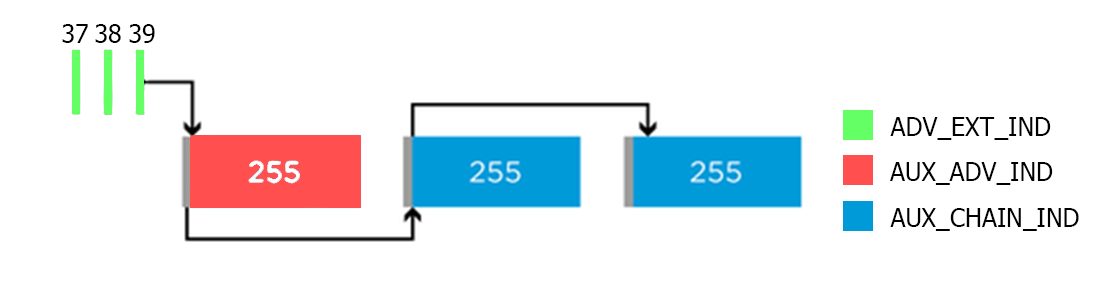
\includegraphics[width=1\textwidth]{./images/aux_chain_ind.png}
		\caption{Exemple d'anunci estès \cite{adv_ext}}
		\label{fig:aux_chain_ind}
	\end{center}
\end{figure}

Un cop explicats els paquets per separat, s'explicarà un exemple de com s'utilitzen aquests paquets per transmetre tanta informació com es vulgui sense necessitat d'establir una connexió.
En primer lloc, l'anunciador envia pels canals d'anunci (habitualment s'envia múltiples vegades per cada canal primari) l'ADV\_EXT\_IND.
Posteriorment, es transmet pel canal secundari l'AUX\_ADV\_IND que indica quan i on es transmetrà el següent paquet.
Finalment, es transmeten tants AUX\_CHAIN\_IND com siguin necessaris fins que s'hagi enviat totes les dades d'anunci que es vulgui.


\subsection{Paràmetres}
BLE permet seleccionar qualsevol combinació de canals per on transmetre els anuncis.
Per consumir menys energia es pot transmetre en un únic canal però això es recomana no fer-ho, ja que si el canal és sorollós, els dispositius no el podran detectar.

Un paràmetre molt important que es pot configurar és l'interval d'anunci.
Aquest valor defineix el temps que passa entre que es transmeten anuncis pel mateix canal tal com es pot veure en la Figura \ref{fig:advertisment_params}.
L'especificació de BLE defineix que pot estar entre 20 ms i 10.24 s amb salts de 0.625 ms.
Aquest paràmetre és crític depenent del servei que es vol oferir.
Si el valor és molt alt, ajudarà a reduir el consum d'energia considerablement però això augmentarà la latència de descobriment de dispositius.

Un cop s'estableix la connexió ja es poden enviar dades ràpidament però per l'escaneig són necessaris múltiples intervals d'anunci i cal considerar que és possible que el receptor no detecti tots els anuncis. 
És per això que, quan es desenvolupen serveis que interaccionen amb persones no és acceptable haver d'esperar desenes de segons, per tant, habitualment s'utilitzen valors d'entre 100 i 500 ms.
En canvi, per a dispositiu que requereixen la mínima latència possible en les dades s'utilitzen valors entre 20 i 50 ms.
Finalment, aquells dispositius que proporcionen dades que no varien sovint i que no requereixen interacció utilitzen valors des d'1 fins a 5 segons.

\begin{figure}[h!]
	\begin{center}
		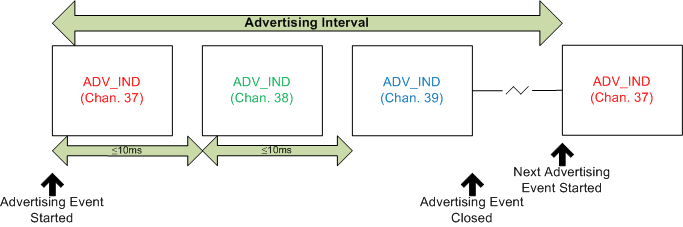
\includegraphics{./images/advertisement_params.png}
		\caption{Paràmetres d'anunci \cite{advertisment_params}}
		\label{fig:advertisment_params}
	\end{center}
\end{figure}

Tot i que, es pot definir el valor de l'interval d'anunci cal tenir en compte que segons l'especificació de BLE s'aplica un retard pseudoaleatori que pot ser de fins a 10 ms i afecta els serveis que requereixen molt poca latència.
Aquest retard aleatori s'implementa per evitar col·lisions entre dispositius que s'han sincronitzat involuntàriament i tenen el mateix interval o un múltiple entre si.

Fins ara s'ha parlat de definir un únic valor d'interval d'anunci, però habitualment, s'estableix un règim on es va canviant aquest valor depenent de la situació.
Quan el dispositiu s'encén o quan s'espera una connexió es disminueix l'interval d'anunci per tal que la connexió s'estableixi més ràpidament.
En canvi, quan fa temps que no hi ha cap connexió s'augmenta l'interval d'anunci per reduir el consum d'energia. 


\section{Escaneig}
Quan un dispositiu es vol anunciar, a part de transmetre anuncis, també ho pot fer fent escaneigs a dispositius que s'han anunciat prèviament.
El procés d'escanejar en l'especificació de BLE 5 s'anomena \textit{Device Discovery} i es basa en dos tipus, l'escaneig actiu i el passiu.
En cas de fer escaneig passiu només es pot obtenir informació a través dels anuncis d'altres dispositius.
Si l'escaneig és actiu, es poden enviar requeriments d'escaneig per demanar informació addicional a la qual hi ha als anuncis.


\subsection{Tipus}
Per a l'escaneig actiu hi ha dos paquets en la versió 4.0 i BLE 5 n'afegeix dos més.
l'SCAN\_REQ serveix per requerir més informació a un dispositiu que s'està anunciant i que accepta aquest tipus de petició.
En el paquet no hi van dades pròpies, només s'hi indica l'origen i destí.
L'SCAN\_RSP és la resposta al paquet anterior, conté l'adreça pròpia de l'anunciador i fins a 31 bytes de dades.
L'extensió que aporta BLE 5 defineix 2 nous tipus de paquets, l'AUX\_SCAN\_REQ i l'AUX\_SCAN\_RSP que tenen la mateixa funcionalitat que els anteriors respectivament.
La diferència és que serveixen per a les comunicacions a través de canals secundaris.
Conseqüentment la quantitat de dades passa a ser de fins a 254 bytes en la resposta.

\subsection{Paràmetres}
Els paràmetres d'escaneig es poden identificar en la Figura \ref{fig:escaneig_canals}.

\begin{figure}[!h]
	\begin{center}
		\begin{subfigmatrix}{1}
			\subfigure[Escaneig de canals]{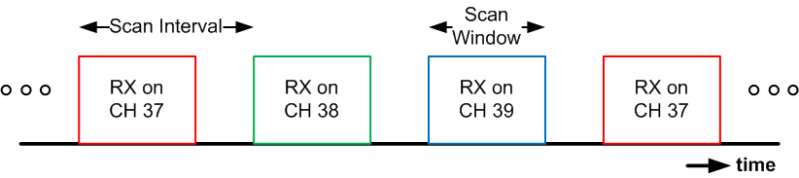
\includegraphics[width=0.9\textwidth]{./images/scanning_diagram}}
			\subfigure[Periodes d'escaneig]{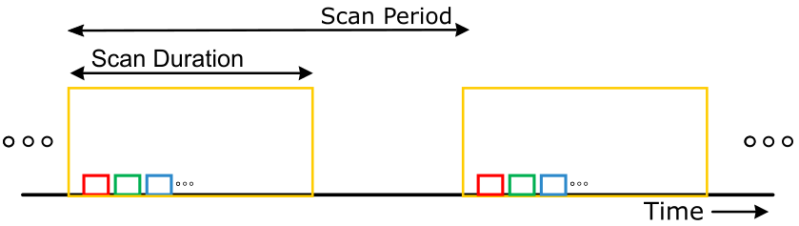
\includegraphics[width=0.9\textwidth]{./images/scanduationperiod}}
		\end{subfigmatrix}
	\end{center}
	\caption{Paràmetres d'escaneig \cite{advertisment_params} }
	\label{fig:escaneig_canals}
\end{figure}

L'interval d'escaneig és el temps des que es comença a escanejar en dos canals consecutius, es pot definir entre 10 ms i 10,24 s.
La finestra d'escaneig és el temps en què s'està escoltant a un canal.
Duració d'escaneig, és el temps que el dispositiu estarà escanejant.
Es pot configurar des de 10 ms fins a 65 segons o escaneig indefinit.
El període d'escaneig indica el temps entre que comencen les duracions d'escaneig i que serveix per poder fer pauses en què el dispositiu no escaneja.


\section{Connexions}
S'ha vist com no cal establir una connexió per a transmetre poca informació.
Això permet desenvolupar implementacions molt simples per a situacions on es transmet amb molt poca freqüència.
Tot i això, BLE també permet transmetre moltes més dades quan s'estableix una connexió.

Un cop s'hagi establert la connexió es podrà transmetre la informació molt eficientment, però establir una connexió suposa un cost energètic considerable.
Per tant, a l'hora de definir els paràmetres de la connexió és important evitar, a ser possible, establir connexió cada vegada que es vol transmetre informació.

Com que les connexions estan basades en múltiples esdeveniments en instants determinats es considerà una connexió síncrona.
No hi ha límit de connexions segons l'especificació de BLE i per tant, dependrà de les capacitats del dispositiu amb el qual es treballa.

Cal recordar que, per crear una connexió és necessari que un dispositiu tingui el rol GAP de central i un altre amb el rol de perifèric (els anunciadors i observadors no poden iniciar connexions).

El dispositiu central serà el que iniciarà la connexió i el perifèric el que l'acceptarà o no.
El central serà sempre el mestre i el perifèric serà l'esclau de la connexió.
Per iniciar una connexió el mestre envia un missatge de tipus CONNECT\_IND\footnote{Aquest paquet en la versió 4 de BLE s'anomena CONNECT\_REQ} amb els paràmetres de la connexió.
En aquests paràmetres, tal com es veurà més endavant en l'apartat \ref{sec:params}, hi ha la informació necessària per determinar el primer esdeveniment de la connexió.
En cada esdeveniment, els dos dispositius tenen un temps assignat per transmetre i per rebre dades.

\begin{figure}[!h]
	\begin{center}
		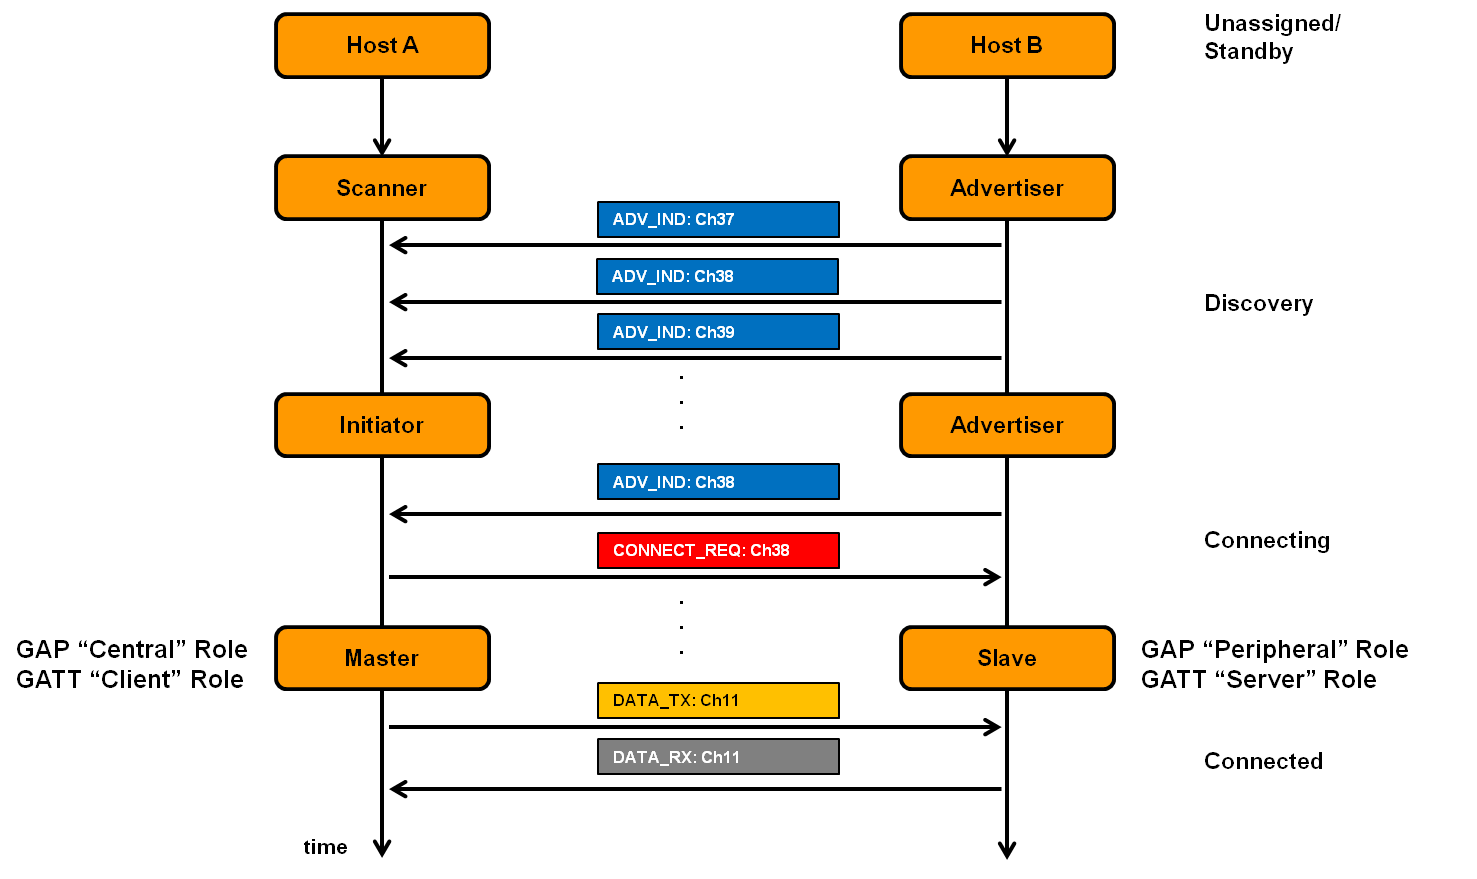
\includegraphics[width=1\textwidth]{./images/rols_unicast.png}
		\caption{Establiment de connexió \cite{fig:connection_establishement}}
		\label{fig:unicast_roles}
	\end{center}
\end{figure}


A la Figura \ref{fig:unicast_roles} es pot observar el procediment en que dos dispositius estableixen una connexió.
Tenim el dispositiu A que, inicialment, està com a observador i el dispositiu B que s'està anunciant.
Cal recordar que, els anuncis no es detecten tots, ja que els dispositius no sempre estan transmetent i escoltant en el mateix canal primari.

El dispositiu A decideix establir una connexió amb el dispositiu B i envia un requeriment de connexió en l'últim canal en que s'ha escoltat l'anunci.
El dispositiu B després de transmetre un anunci per un canal, escolta durant un temps determinat en el mateix canal a l'espera de requeriments de connexió.
Quan el dispositiu B rep el requeriment, decideix acceptar la connexió i respon a aquest.

En aquest moment, el dispositiu A passa a ser el mestre amb els rols Central i Client i el dispositiu B passa a ser l'esclau amb rols de perifèric i servidor.
La connexió està establerta i ja és possible transmetre dades entre ambdós dispositius durant els esdeveniments de connexió. 


\subsection{Paràmetres}
\label{sec:params}
L'interval de connexió és un dels paràmetres més importants en la connexió BLE, estableix com de sovint es comuniquen els dispositius.
És el temps que hi ha entre esdeveniments de la connexió i va entre 7,5 ms i 4 s.
Com que el que es configuren són preferències, es determina l'interval mínim i el màxim que es vol.
En cas que es vulgui fixar, simplement, s'ha d'indicar el mateix valor per al mínim i al màxim.

BLE permet a l'esclau saltar-se esdeveniments per tal d'estalviar bateria, per exemple, si no té dades a transmetre.
La latència de l'esclau, que és un dels paràmetres de connexió, defineix la quantitat màxima d'esdeveniments que l'esclau pot saltar i que la connexió segueixi establerta.

En la Figura \ref{fig:slave_latency} es pot observar la comparació entre quan s'utilitza la latència d'esclau i quan no.
Tot i això, el mestre que és el node que té més bateria, participa en tots els esdeveniments escoltant el canal per si l'esclau transmet.
Utilitzar aquest paràmetre permet tenir una connexió amb una latència baixa però amb un consum igualment reduït mentre no s'hagin de transmetre dades molt sovint.

\begin{figure}[!h]
	\begin{center}
		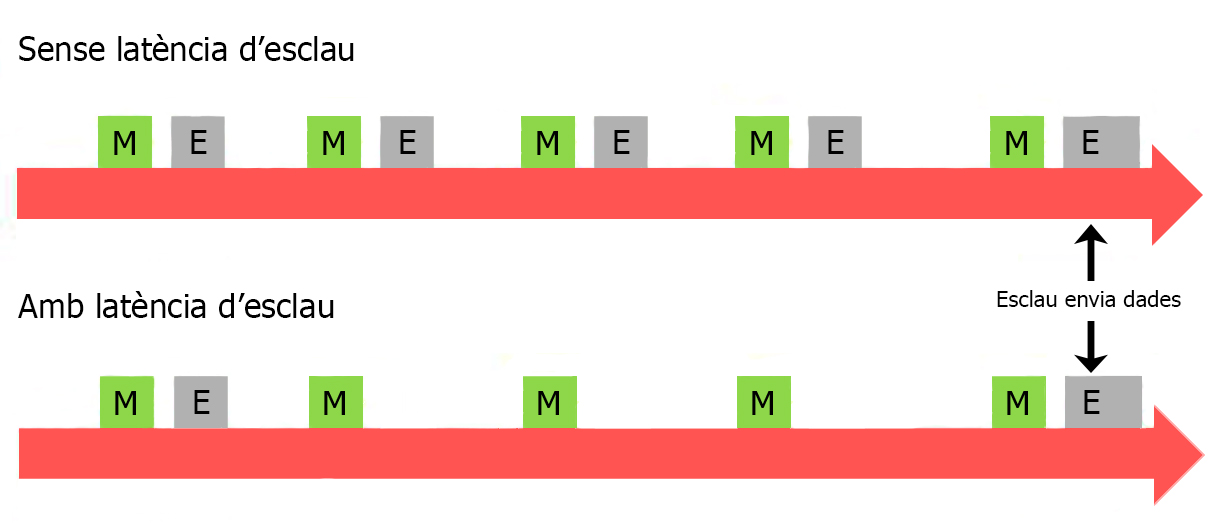
\includegraphics{./images/slave_latency_new.jpeg}
		\caption{Comparació d'esdeveniments amb latència d'esclau \cite{slave_latency}}
		\label{fig:slave_latency}
	\end{center}
\end{figure}

L'últim paràmetre és el temps de supervisió, és el temps màxim acceptable que pot passar sense activitat en la connexió.
Si es supera aquest temps, es considera que la connexió s'ha acabat i per tant, per comunicar-se s'ha de tornar a iniciar.
Això pot passar, per exemple, en entorns molt sorollosos o més sovint quan els dispositius surten del seu abast i el senyal no és detectable.

\section{Seguretat}
\label{sec:security}
Com que l'ús de BLE és molt flexible, per poder-lo utilitzar en certes aplicacions es requereix que l'intercanvi de dades sigui segur.
Això significa que la connexió tingui resistència a atacs d'\textit{eavesdrop}\footnote{Aquest tipus d'atac permet a l'atacant conèixer el contingut dels missatges que es transmeten.} passiu i d'intermediari\footnote{Aquest tipus d'atac permet modificar la informació que es transmet sense que sigui evident pel transmissor o el receptor.} (\textit{Man In The Middle} en anglès).
BLE utilitza l'encriptació simètrica AES-CCM, però la seguretat rau en com els nodes s'intercanvien la clau.

Hi ha diferents maneres que el desenvolupador pot escollir utilitzar i que varien en seguretat i facilitat d'ús.
Existeix el mètode sense seguretat anomenat \textit{Just Works}.
Aquest mètode és útil en casos on no es requereix seguretat o que no és possible tenir-ne per les limitacions del dispositiu amb el qual es vol establir connexió.

Un altre mètode és l'\textit{Out of Band}, aquest permet utilitzar una altra tecnologia per l'intercanvi de claus, com per exemple, NFC (comú en auriculars d'alta gamma).
La seguretat d'aquest mètode depèn completament en el nou sistema per l'intercanvi de claus.

El més habitual és el \textit{Passkey} en què l'intercanvi de claus es bassa en una contrasenya de 4 a 6 dígits.
Cal tenir en compte que, a causa del baix nombre de combinacions depenent de la implementació aquest mètode serà sensible a atacs d'\textit{eavesdropping} passiu.

Finalment, un mètode similar l'anterior és el de Comparació Numèrica, en lloc de ser l'usuari qui introdueix el codi es genera automàticament i es mostra en els dos dispositius.
Cal comprovar que sigui el mateix número en els dos casos i això permet prevenir atacs de \textit{Man in the Middle} però, de nou, no protegeix contra l'\textit{eavesdropping}.

\section{Format}
\label{sec:format}
En aquest apartat s'explicarà com estan formats els paquets que s'envien en BLE i de quins camps estan formant.
Cal distingir però entre la versió 4.2 i la 5 de BLE, ja que degut a les noves funcionalitats, el format canvia considerablement.

\subsection{BLE 4.2}
En la versió de BLE 4.2\footnote{En les versions anteriors a la 4.2 la PDU tenia una mida màxima de 39 bytes.} els paquets que es transmeten segueixen el format de la Figura \ref{fig:4_2_format}.

\begin{figure}[!h]
	\begin{center}
		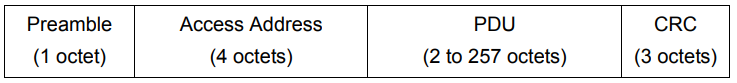
\includegraphics[width=1\textwidth]{./images/Packet_format_4_2.png}
		\caption{Format del paquet en BLE 4.2 \cite{BLE_4.2_packet_format}}
		\label{fig:4_2_format}
	\end{center}
\end{figure}

El preàmbul és una seqüència predefinida i que serveix per sincronisme.
L'adreça d'accés identifica a quina connexió pertany aquest paquet, en cas de ser d'anunci i no pertànyer a cap connexió el valor és 0x8E89BED6.
Aquest camp serveix al receptor per filtrar els paquets i només tractar aquells que interessa.
El CRC (Cyclic Redundancy Check) s'utilitza per detectar errors en el paquet. 

En la PDU (Protocol Data Unit) és on es troba la informació pròpia del paquet i depenent de si és un paquet en un canal d'anunci o en un de dades té un format lleugerament diferent.
En la Figura \ref{fig:pdu_format} es poden veure les diferències.
Cal destacar que, en el cas de ser un anunci tot l'espai es dedica a informació, en canvi, en la PDU d'anunci es reserven 4 bytes per al comprovant d'integritat del missatge (\textit{Message Integrity Check} en anglès).

\begin{figure}[!h]
	\begin{center}
		\begin{subfigmatrix}{1}
			\subfigure[Format PDU d'anunci \cite{BLE_4.2_packet_format}]{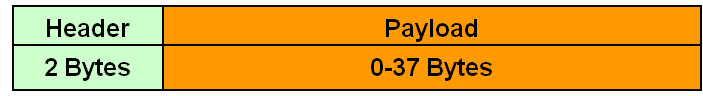
\includegraphics[width=0.8\textwidth]{./images/Packet_format_4_2_adv.png}}
			\subfigure[Format PDU de dades \cite{BLE_4.2_packet_format}]{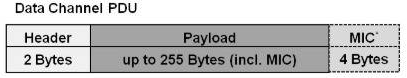
\includegraphics[width=0.8\textwidth]{./images/Packet_format_4_2_data.png}}
		\end{subfigmatrix}
	\end{center}
	\caption{Format PDU}
	\label{fig:pdu_format}
\end{figure}

Pel que fa a la Càrrega Útil (\textit{Payload}) serà diferent segons el tipus de paquet.
En el cas de l'ADV\_IND està format per l'adreça de l'anunciant seguit d'un llistat d'estructures de dades d'anunci (\textit{Advertisement Data Structure}).
Aquestes, estan formades per la longitud de l'estructura, el tipus i les dades en si.
Existeixen molts tipus d'estructura que estan definits en l'estàndard \cite{AD_Types}.

\begin{figure}[!h]
	\begin{center}
		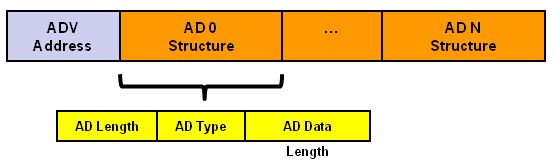
\includegraphics[width=0.8\textwidth]{./images/adv-ind-packet.png}
		\caption{Payload de ADV\_IND \cite{BLE_4.2_packet_format}}
	\end{center}
\end{figure}

En canvi, en el cas de l'ADV\_DIRECT\_IND simplement s'indica l'adreça de l'anunciador i la del dispositiu al qual va dirigit el paquet.

\subsection{BLE 5}
Els canvis per a BLE 5 corresponen a les noves possibilitats que s'han comentat a l'apartat \ref{Versions_BLE}.
Primer, la funcionalitat per poder transmetre anuncis als canals secundaris que s'ha comentat a \ref{Advertisement_Extensions} i enumerat els tipus de paquets a \ref{Advertising_Extension_PDU}

\begin{figure}[!h]
	\begin{center}
		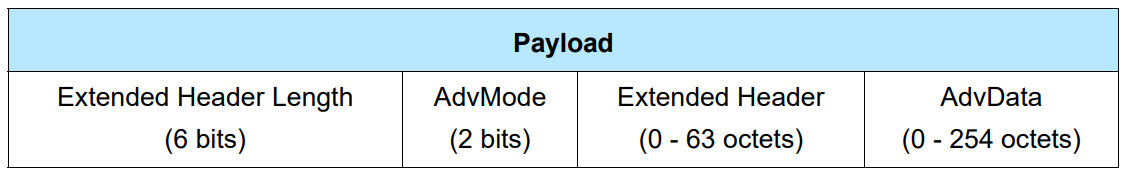
\includegraphics[width=0.9\textwidth]{./images/Common_Extended_Advertising_Payload_Format.png}
		\caption{Format de la Extended Advertising Payload \cite{BLE_5_Extended_Advertising}}
	\end{center}
\end{figure}

Tots els paquets nous de BLE 5 d'anunci es basen en aquest format flexible.
L'\textit{Extended Header Length} defineix la longitud de l'\textit{Extended Header}.
L'\textit{AdvMode} defineix una sèrie de valors que identifiquen si l'anunciador accepta connexions o es pot escanejar.
L'\textit{Extended Header} indica informació similar a la versió 4.2 com l'adreça de l'anunciador.
Però també indica tot el necessari per BLE 5, com en quin canal secundari es transmetrà part de la informació del paquet o amb quin tipus de capa física es transmetrà aquesta informació (LE 1M, LE 2M o LE Coded) entre d'altres.

\section{Xarxes Bluetooth multi-node}
Tal com s'ha vist anteriorment, el Bluetooth Low Energy només permet tenir connectivitat punt a punt i això no és suficient per poder competir amb les altres tecnologies.
Si tenim un node que es connecta amb múltiples dispositius BLE, aquests no es poden comunicar entre si i això limita l'ús de BLE en grans desplegaments.
D'altre banda, les altres MANETs que s'han vist a l'apartat \ref{MANETS}; com Zigbee, 6LoWPAN o Z-Wave, entre d'altres, estableixen mecanismes que permeten connectar tots els nodes entre si a través d'una xarxa.

Bluetooth necessitava definir algun mètode oficial per poder implementar xarxes complexes entre nodes i ho va fer amb el \textit{Mesh Profile}.
El juliol del 2017 es va adoptar l'estàndard del perfil de malla (\textit{Mesh Profile} en anglès) format per la definició del perfil \cite{Mesh Profile Definition} i per la definició del models \cite{Mesh Profile Models}.

Aquest estàndard és molt rellevant per a BLE, ja que anteriorment l'abast màxim dels dispositius estava estrictament limitat.
En canvi, amb l'ús del \textit{Mesh Profile} és possible estendre la connectivitat amb nodes intermedis que facin de repetidors.
Però aquesta no és l'únic avantatge que aporta, a continuació es descriurà resumidament com funciona el \textit{Mesh Profile} i com ajuda a augmentar les capacitats de BLE.

\subsection{Topologia}
Bluetooth té definicions per a diferents tipologies de nodes que es poden observar a la Figura \ref{piconet}.

\begin{figure}[!h]
	\begin{center}
		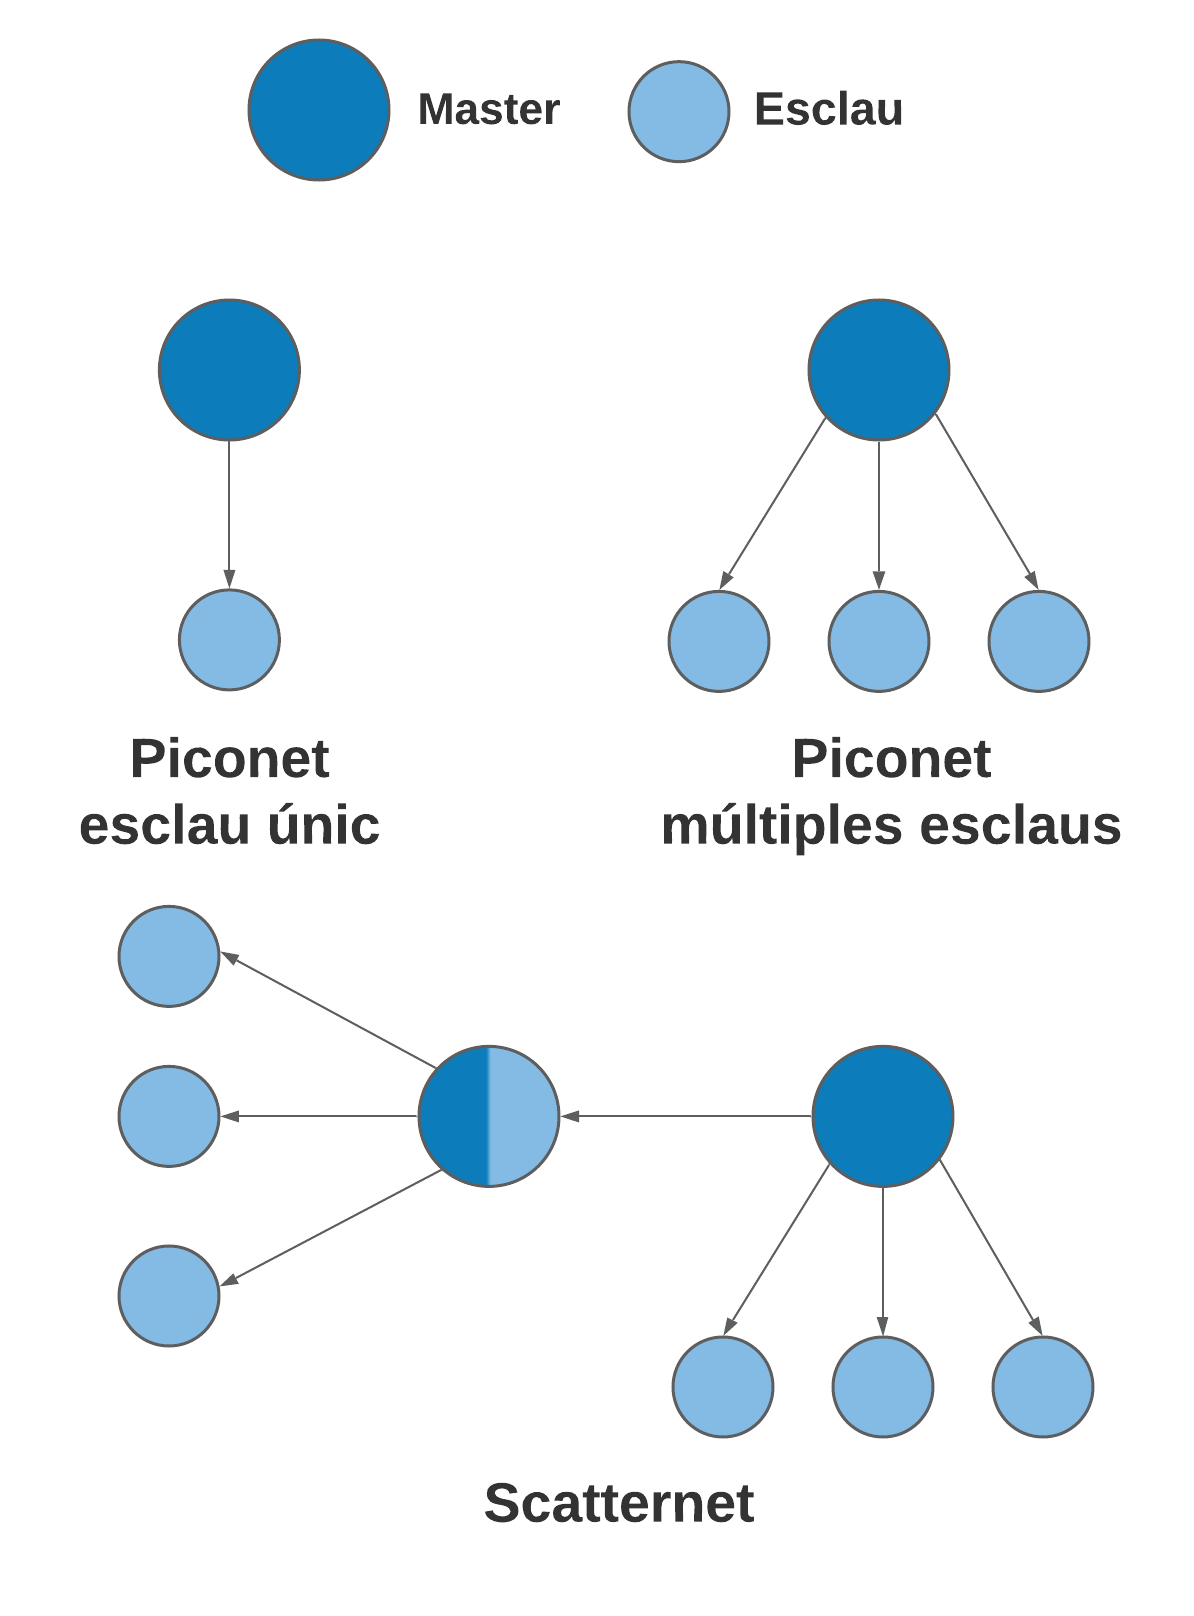
\includegraphics[width=0.6\textwidth]{./images/PICONET.png}
		\caption{Tipus de xarxes}
		\label{piconet}
	\end{center}
\end{figure}

En Bluetooth Clàssic els missatges que s'envien tenen un únic node origen i un únic node destí i per tant formen una \textit{Piconet} d'esclau únic.
Amb la introducció de BLE sorgeix la possibilitat d'enviar un mateix missatge amb potencialment múltiples dispositius com a destí, per exemple, utilitzant missatges d'anunci.
Aquestes d'interaccions són punt a multipunt, és a dir, un mestre pot estar connectat a més d'un esclau, però un esclau només estarà connectat a un mestre.
Aquest tipus de xarxa s'anomena \textit{Piconet} d'esclaus múltiples.

Gràcies al nou \textit{Mesh Profile} un node pot ser mestre en una connexió i esclau en una altra.
D'aquesta manera els nodes formen connexions multipunt a multipunt, és a dir, un mateix node pot estar connectat amb esclaus i mestres a la vegada.
Aquesta tipologia de xarxa està formada per múltiples \textit{piconets} interconnectades i en conjunt s'anomena \textit{scatternet}.

Pel reenviament dels paquets en lloc d'utilitzar protocols d'encaminament basats en IP s'utilitza encaminament d’inundació gestionat (\textit{managed flood routing}, en anglès).
L'ús d'aquest protocol és per fer el més simple possible el desenvolupament de dispositius així com reduir el sobrecost en processament i memòria.

És molt comú que es vulguin canviar múltiples elements a la vegada com poden ser llums, temperatura del termòstat i persianes.
Per reduir la quantitat de missatges enviats es poden utilitzar escenes que permeten interactuar amb múltiples nodes a la vegada.
Aquestes escenes es poden activar a través d'un únic missatge o també es poden programar perquè s'activin automàticament a una certa hora.

Cal destacar que, tot i que probablement la majoria de xarxes que utilitzin el \textit{Mesh Profile} no seran molt grans, l'estàndard s'ha dimensionat per poder tenir xarxes extremadament grans, pensades per pàrquings de cotxes, control d'il·luminació en edificis d'oficines o sensors en caps de futbol entre d'altres.
Els límits són de 32.767 nodes per xarxa, fins a 4.096 subxarxes i 65.535 escenes, i vénen marcats per la longitud dels camps corresponents que són de 15, 12 i 16 bits respectivament.

\begin{figure}[!h]
	\begin{center}
		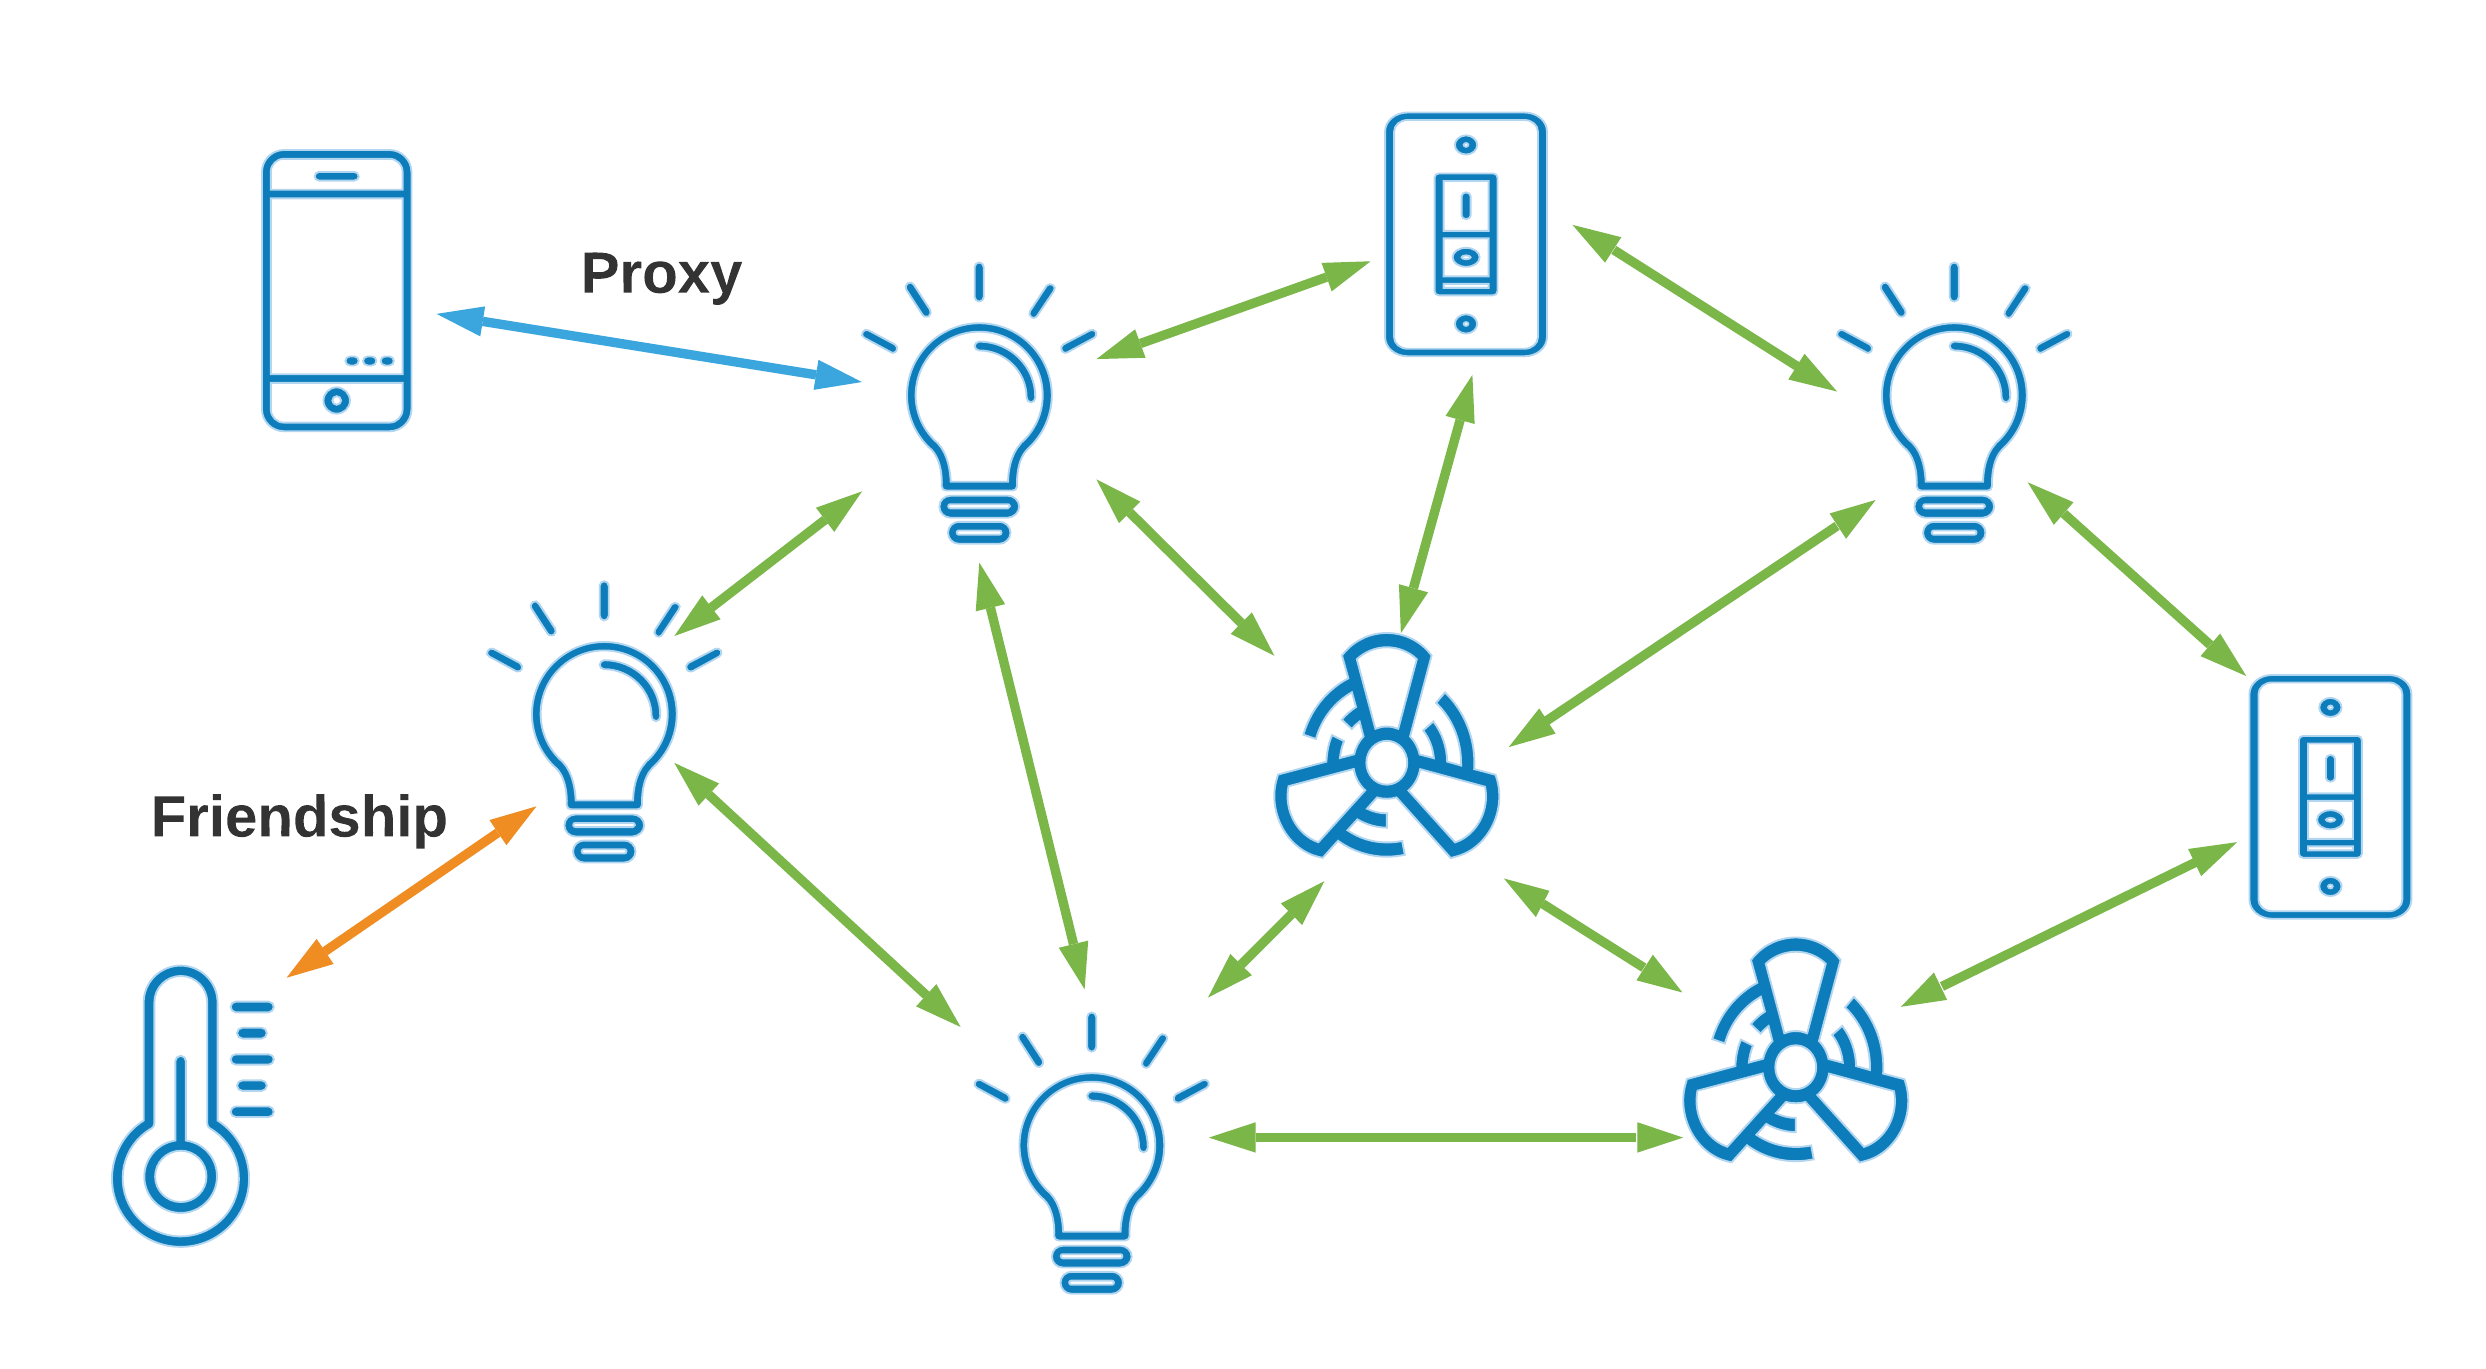
\includegraphics[width=0.8\textwidth]{./images/mesh_profile_features.png}
		\caption{Exemple \textit{Mesh Profile} \cite{Mesh Profile}}
	\end{center}
\end{figure}

Per facilitar la introducció del \textit{Mesh Profile} en desplegaments de BLE ja existents es defineix un mode d'operació intermediari (\textit{proxy}, en anglès).
El mode intermediari permet a un node d'una xarxa establir una connexió utilitzant BLE amb un altre node que no implementa el \textit{Mesh Profile}.
Així, un node antic pot ser perfectament controlat a través d'una \textit{Scatternet}.

Tenir una xarxa de nodes que reenvien paquets quan alguns dels nodes són de baix consum i amb poca capacitat de processament pot suposar problemes.
És per això que, el \textit{Mesh profile} inclou la possibilitat de definir una connexió d'amistat on el node de baix consum és l'amic.
Aquest dispositiu amic no haurà d'estar escoltant constantment sinó que podrà requerir els paquets dirigits a ell quan es desperti.
L'altre node associat que tindrà més capacitat de processament, memòria i probablement estarà connectat a la xarxa elèctrica haurà d'emmagatzemar els paquets i reenviar-los quan siguin requerits.

\subsection{Pila}
El \textit{Mesh Profile} defineix les capes de la seva pròpia pila.
En la capa inferior d'aquesta pila hi conté tot BLE, ja que el \textit{Mesh Profile} utilitza BLE per enviar paquets entre els nodes que formen la xarxa.
A continuació, es comentarà breument les diferents capes.

\begin{figure}[!h]
	\begin{center}
		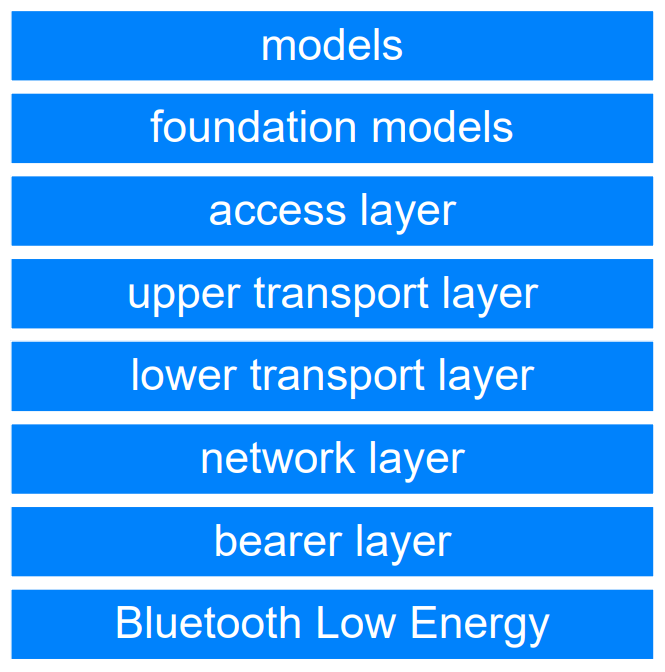
\includegraphics[width=0.6\textwidth]{./images/mesh_profile_stack2.PNG}
		\caption{Arquitectura del \textit{Mesh Profile} \cite{Mesh Profile Overview}}
		\label{mesh_netowrk_stack}
	\end{center}
\end{figure}

La capa \textit{Bearer} controla la transmissió i recepció de paquets, hi ha dos tipus, l'\textit{Advertising Bearer} i el GATT \textit{Bearer}.
L'\textit{Advertising Bearer} utiliza el BLE per enviar i rebre missatges corresponents al \textit{Mesh Profile}.
En canvi, el GATT \textit{Bearer} és el que s'utilitza per interactuar amb dispositius que no implementen el \textit{Mesh Profile} utilitzant el protocol d'intermediari comentat anteriorment.

La capa de xarxa defineix l'ús d'adreces i la gestió de les múltiples interfícies que pot tenir un node.
Les funcions de repetidor s'implementen en aquesta capa.
La capa de transport inferior realitza la segmentació i reassemblatge dels paquets que no caben en una PDU de transport.
La capa de transport superior és responsable de la seguretat, proveeix encriptació i autenticació.
Igualment, també s'encarrega de la funcionalitat d'amistat entre dispositius comentada anteriorment.
En la capa d'accés es defineix el format de les dades de la capa de transport incloent quina encriptació s'ha de realitzar entre d'altres.
Les dues capes superiors tracten la implementació dels models, els missatges i estats que defineix l'estàndard.

Comparant les capes de \textit{Mesh Profile} i de BLE (Figura \ref{controller_stack} i Figura \ref{host_stack}) es pot observar que són similars fins al punt que s'estan realitzant les mateixes funcions.
Això es deu al fet que en lloc de substituir o estendre BLE amb el \textit{Mesh Profile}, el que s'ha fet és mantenir BLE tal com està i afegir \textit{Mesh Profile} per sobre.
D'aquesta manera s'assegura la compatibilitat entre dispositius que implementen el \textit{Mesh Profile} i dispositius que no.
A més a més, és compatible amb BLE 5 i amb BLE 4, així que és molt fàcil afegir dispositius amb \textit{Mesh Profile} en una instal·lació ja existent.

\subsection{Seguretat}
En la majoria de tecnologies que s'han vist fins ara, incloent-hi BLE la seguretat és opcional per permetre implementacions simples del protocol que no la requereixen.
Aquest no és el cas del \textit{Mesh Profile} que obliga a utilitzar seguretat segons l'estàndard.

Tots els paquets corresponents al \textit{Mesh Profile} estan encriptats i autenticats.
Per fer-ho existeixen les claus de xarxa que són compartides entre tots els nodes de la mateixa xarxa i es requereixen per realitzar funcions de xarxa com reenviar paquets.
Amb aquestes claus s'ofusquen les capçaleres del paquet per donar privacitat de l'origen i destí envers un potencial actor maliciós que no pertany a la xarxa.
Si un node forma part d'una subxarxa, aquest també tindrà una altra clau única i compartida entre els nodes de la subxarxa.
Per tant, es poden aïllar certes parts de la xarxa, per exemple, una estança d'un d'hotel.

Cada xarxa pot tenir múltiples aplicacions que tindran la seva pròpia clau d'aplicació.
Aquesta servirà per aïllar diferents elements d'una xarxa que estan relacionats com poden ser els elements d'il·luminació (llums i interruptors) dels elements de calefacció (sensor de temperatura i radiador).

Finalment, tots els nodes contenen una clau de dispositiu que els permet formar part d'una xarxa o una aplicació.
Quant un dispositiu es vol eliminar de la xarxa o aplicació, per exemple, per vendre'l, es procedeix de forma segura afegint aquella clau a una llista negra.
Els dispositius que estan a la llista negra no se'ls renoven les claus d'aplicació o xarxa i per tant no poden seguir participant en les comunicacions.
Tal com és habitual s'utilitzen identificadors seqüencials en els paquets per evitar atacs de repetició on l'atacant retransmet un paquet per intentar repetir una acció anterior.

